\section{Helicopter Specific Design}
Consider the application of the combined inner-outer-loop adaptive
architecture to the trajectory control of a helicopter. The dynamics
\cite{munzinger:masters,mettler,gavrilets:gnc:01} of the helicopter
may be modeled in the same form as \eqrng{e:pdot}{e:omdot}. Most
small helicopters include a \label{r:bellhillier}Bell-Hiller
stabilizer bar, which provides provide lagged rate feedback, and is a
source of unmodeled dynamics. The nonlinear model used for simulation
in this work included the stabilizer bar dynamics. Additionally,
blade flapping and other aspects such as gear and engine dynamics
were also modeled.
%
\subsection{Approximate Model}
An approximate model for the attitude dynamics of the helicopter was
generated by linearizing the nonlinear model around hover and
neglecting coupling between the attitude and translational dynamics
as well as the stabilizer bar
\begin{align}
\label{e:attinverse} \aldes &= \hat{A}_1
\begin{bmatrix}
p \\ q \\ r
\end{bmatrix}
+ \hat{A}_2
\begin{bmatrix}
u \\ v \\ w
\end{bmatrix}
+ \hat{B} \left( \underbrace{\begin{bmatrix} \delta_{lat} \\
\delta_{lon} \\ \delta_{ped}
\end{bmatrix}}_{des}
- \underbrace{\begin{bmatrix} \delta_{lat} \\ \delta_{lon} \\
\delta_{ped}
\end{bmatrix}}_{trim}
\right),
\end{align}
or,
\[
\aldes = \hat{A}_1\bfomega_B + \hat{A}_2\bfv_B + \hat{B}(\delmdes -
\bfdelta_{m_{trim}}).
\]
%
where, $\hat{A}_1$ and $\hat{A}_2$ represent the attitude and
translational dynamics respectively, $\bfomega_B$ represents the
angular velocity of the body with respect to the earth expressed in
the body frame. The body velocity velocity vector with respect to the
earth expressed in the body frame is given by $\bfv_B$ and
$\bfdelta_{m_{trim}}$ is the trim control vector that is consistent
with the linear model.
%
Choosing the control matrix $\hat{B}$ such that it is invertible,
the moment controls may be evaluated as
%
\[
\delmdes = \hat{B}^{-1}(\aldes - \hat{A}_1\bfomega_B - \hat{A}_2
\bfv_B) + \bfdelta_{m_{trim}}.
\]
%
\begin{figure}
  \centering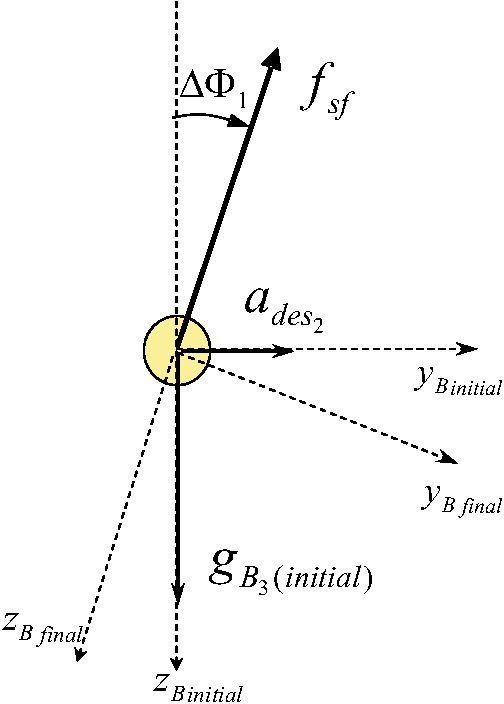
\includegraphics[width=0.4\columnwidth]{pointmass}
%  \centering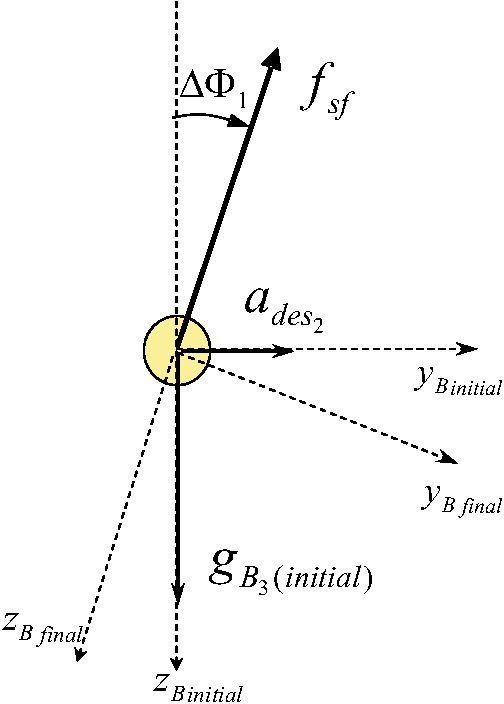
\includegraphics{pointmass}
  \caption{Point mass model for outerloop inversion.}
  \label{f:pointmass}
\end{figure}
%
The translational dynamics may be modeled as a point mass with a
thrust vector that may be oriented in a given direction as
illustrated in \fig{f:pointmass}. More involved inverses
\cite{lipp:mcm:1993} may be used, but the simple relationships between
thrust, attitude and accelerations suffice when used with adaptation
%
\begin{equation}
\label{e:transinverse} \ades =
\begin{bmatrix}
0 \\ 0 \\ Z_{\delta_{coll}}
\end{bmatrix}
\left(
\delta_{coll_{des}} - \delta_{coll_{trim}}
\right)
 + L_{bv}\bfg,
\end{equation}
where, $Z_{\delta_{coll}}$ is the control derivative for
acceleration in the vertical axis. $L_{bv}$ is the direction cosine
matrix that transforms a vector from the vehicle (or local) frame to
the body frame and $\bfg$ is an assumed gravity vector. The desired
specific force along the body $z$ axis may be evaluated as
\[
f_{sf} = (\ades - L_{bv}\bfg)_3.
\]
%
The required collective input may be evaluated as
\[
\delta_{coll_{des}} = \frac{f_{sf}}{Z_{\delta_{coll}}} +
\delta_{coll_{trim}}.
\]
%
The attitude augmentation required in order to orient the thrust
vector to attain the desired translational accelerations are given
by the following small angle corrections from the current
reference body attitude and attitude command
%
\begin{align}
\label{e:DelPhi}
\Delta\Phi_1  = \frac{a_{des_2}}{f_{sf}},\quad%
\Delta\Phi_2  = -\frac{a_{des_1}}{f_{sf}},\quad%
\Delta\Phi_3  = 0,%
\end{align}
For this simplified helicopter model, heading change has no effect
on accelerations in the $x,y$ plane and hence $\Delta\Phi_3 = 0$.
These three correction angles may now be used to generate the
attitude quaternion correction desired by the outer loop. Thus,
%
\begin{equation}
\label{e:qdessmallangle} \qdes =
\bfq(\Delta\Phi_1,\Delta\Phi_2,\Delta\Phi_3),
\end{equation}
where, $\bfq(.)$ is a function\cite{stevens2003} that expresses an
euler-angles-based rotation as a quaternion. The overall detailed
controller architecture is shown in \fig{f:detailarch}.
%

%
\begin{remark}
If the desired specific force $f_{sf}$ is close to zero, which
occurs when the desired acceleration in the body $z$ axis is the
same as the component of gravity vector along that axis, then,
Equation (\ref{e:DelPhi}) is undefined. To overcome this problem,
one can impose a restriction where \sys{e:DelPhi} is only computed
if $| f_{sf}| > \bar{f}_{sf}$, where $\bar{f}_{sf}
> 0$ and is a lower limit. Essentially it means, do not bother
using attitude unless the desired specific force is greater than
$\bar{f}_{sf}$.
\end{remark}
%
%
\subsection{Reference Model}
\label{s:helirefmodel}
Using a linear $\acrm$ and $\alcrm$ in \eq{e:pddrm} and \eq{e:qddrm} results in the following reference model dynamics
\[
\begin{split}
\dot{\bfv}_{r}      &=  R_p(\pc - \prm) + R_d(\vc - \vrm) - \ah\\
\dot{\bfomega}_{r} &= K_p(\tilde{Q}(\qc\oplus\qdes,\qrm)) + K_d(\oc
- \orm) - \alh,
\end{split}
\]
where, $R_p,R_d,K_p,K_d$ are the same gains used for the PD
compensator in \eq{e:pdgains}. If limits on the angular rate or
translational velocities are to be imposed, then they may be easily
included in the reference model dynamics by choosing the following constrained linear reference for $\acrm$ and $\alcrm$.
\begin{align}
\label{e:acrm}
\acrm    &= R_d[\vc - \vrm + \sigma(\inv{R_d}R_p(\pc - \prm), v_{lim})]\\
\label{e:alcrm}
 \alcrm   &= K_d[\oc - \orm +
\sigma(\inv{K_d}K_p\tilde{Q}(\qc\oplus\qdes,\qrm),\omega_{lim})].
\end{align}
This reference model has prescribable aggressiveness, where $\sigma(\cdot)$ is a saturation function and
$v_{lim}$, $\omega_{lim}$ are the translational and angular rate
limits respectively.

\begin{remark}
\label{rem:vlimwlim}Note that there are no limits placed on the
externally commanded position, velocity, angular rate or attitude.
For example, in the translational reference model, if a large
position step is commanded, $\pc = [1000,0,0]^T ft$ and $\vc =
[0,0,0]^T ft/s$, the speed at which this large step will be achieved
is $v_{lim}$. On the other hand if \mbox{$\pc = \int \vc dt$} and
$\vc = [60, 0, 0]^T ft/s$, the speed of the vehicle will be $60
ft/s$. Similarly, $\omega_{lim}$ dictates how fast large attitude
errors will be corrected. Additionally, aggressiveness with which
translational accelerations will be pursued by tilting the body may
be governed by limiting the magnitude of $\qdes$ to the scalar limit
$q_{lim}$.

\begin{comment}
For large $\ades$, the simple form of the outerloop inversion
will result in very large attitude corrections. Hence, the desired
attitude generated by the outerloop, \eq{e:qdessmallangle}, may be
implemented as
\begin{align}
\lambda &= \frac{q_{lim}}{q_{lim} + max(0,\|\Phi\| - q_{lim})}\\
\qdes   &=
q(\lambda\Delta\Phi_1,\lambda\Delta\Phi_2,\lambda\Delta\Phi_3)
\end{align}
where $q_{lim}$ is a limit on the attitude correction and
\mbox{$\|\lambda[\Delta\Phi_1,\Delta\Phi_2,\Delta\Phi_3]^T\| \leq
q_{lim}$}.
\end{comment}
\end{remark}

%
\subsection{Choice of Gains Linear Dynamics}
\label{s:gainchoice} When the combined adaptive inner-outer-loop
controller for position and attitude control is implemented, the
poles for the combined error dynamics must be selected appropriately.
The following analysis applies to the situation where inversion model
error is compensated for accurately by the NN and it is assumed that the
system is exactly feedback linearized. The inner loop and outer loop
each represent a second order system and the resulting position
dynamics $p(s)/p_c(s)$ are fourth order in directions perpendicular
to the rotor spin axis.

When the closed-loop longitudinal dynamics, near hover, are
considered, and with an acknowledgment of an abuse of notation, it
may be written as
\begin{alignat}{3}
\label{eq:xdd}
\ddot{x} &= a_{des} &=
\ddot{x}_c + R_d(\dot{x}_c - \dot{x}) +
R_p(x_c - x)\\
\label{eq:thdd} \ddot{\theta} &= \alpha_{des} &= \ddot{\theta}_g +
K_d(\dot{\theta}_g - \dot{\theta}) + K_p(\theta_g - \theta),
\end{alignat}
where, $R_p$, $R_d$, $K_p$ and $K_d$ are the PD compensator gains
for the inner loop (pitch angle) and outer loop (fore-aft position).
Now $x$ is now the position, $\theta$ the attitude and $\theta_g$
the attitude command. Normally, $\theta_g = \theta_c + \theta_{des}$
where $\theta_c$ is the external command and $\theta_{des}$ the
outer-loop-generated attitude command. Here, it is assumed that the
external attitude command and its derivatives are zero; hence,
$\theta_g = \theta_{des}$. In the following development, the
transfer function $x(s)/x_c(s)$ is found and used to place the poles
of the combined inner-outer loop system in terms of the PD
compensator gains.

When contributions of $\dot{\theta}_g(s)$ and $\ddot{\theta}_g(s)$,
are ignored, the pitch dynamics \eq{eq:thdd} may be rewritten in the
form of a transfer function as
\begin{equation}
\label{eq:thtf} \theta(s) =
\frac{\theta(s)}{\theta_g(s)}\theta_g(s) = \frac{K_p}{s^2 + K_ds +
K_p}\theta_g(s).
%            \cancel{\frac{\theta(s)}{\dot{\theta}_g(s)}\dot{\theta}_g(s)} +
%            \cancel{\frac{\theta(s)}{\ddot{\theta}_g(s)}\ddot{\theta}_g(s)}
\end{equation}
%
If the outer-loop linearizing transformation used to arrive at
\eq{eq:xdd} has the form $\ddot{x} = f\theta$, where $f = -g$ and
$g$ is gravity, it may be written as
\begin{equation}
\label{eq:xtf} s^2x(s) = f\theta(s).
\end{equation}
The outer-loop attitude command may be generated as
\begin{equation}
\label{eq:thol} \theta_{des} = \frac{\ddot{x}_{des}}{f} =
\frac{a_{des}}{f}.
\end{equation}
Note that $\theta_{g} = \theta_{des}$; if $\theta_c = 0$,
\begin{align}
\label{eq:thetag} \theta_g = \theta_{des} &=
\frac{1}{f}\left[\ddot{x}_c + R_d(\dot{x}_c - \dot{x}) +
R_p(x_c-x) \right].
\end{align}
%
When \eq{eq:thtf} and \eq{eq:thetag} are used in \eq{eq:xtf}
\begin{equation}
\begin{split}
\label{eq:s2x}%
s^2x(s) &= \frac{K_p\left[s^2x_c + R_ds(x_c - x) + R_p(x_c - x)
\right]}{s^2 + K_ds + K_p},
\end{split}
\end{equation}
Rearranging the above equation results in the following transfer function
\begin{equation}
\label{eq:xxctf}
\frac{x(s)}{x_c(s)} =
\frac{K_ps^2 + K_pR_ds + K_pR_p}
{s^4 + K_ds^3 + K_ps^2 + K_pR_ds + K_pR_p}.
\end{equation}

One way to choose the gains is by examining a fourth-order
characteristic polynomial written as the product of two second order
systems
\begin{align}
\label{eq:coeffs2}
\Upsilon(s) &= (s^2 + 2\zeta_o\omega_o + \omega_o^2)(s^2 + 2\zeta_i\omega_i + \omega_i^2) \nonumber \\
&=s^4+(2\zeta_i\omega_i+2\zeta_o\omega_o)s^3 \nonumber \\
&+(\omega_i^2+4\zeta_o\omega_o\zeta_i\omega_i+\omega_o^2)s^2 \nonumber \\
&+(2\zeta_o\omega_o\omega_i^2+2\omega_o^2\zeta_i\omega_i)s
+\omega_o^2\omega_i^2,
\end{align}
where, the subscripts $i$, $o$, represent the inner and outerloop
values respectively.

Comparing the coefficients of the poles of \eq{eq:xxctf} and
\eq{eq:coeffs2} allows the gains to be expressed as a function of
the desired pole locations for each axis in turn
\begin{align}
\label{eq:gains2}
R_p &= \frac{\omega_o^2\omega_i^2}{\omega_i^2+4\zeta_o\omega_o\zeta_i\omega_i+\omega_o^2} \nonumber \\
R_d &=
2\frac{\omega_o\omega_i(\zeta_o\omega_i+\omega_o\zeta_i)}{\omega_i^2+4\zeta_o\omega_o\zeta_i\omega_i+\omega_o^2}
\nonumber \\
K_p &= \omega_i^2+4\zeta_o\omega_o\zeta_i\omega_i+\omega_o^2 \nonumber \\
K_d &= 2\zeta_i\omega_i+2\zeta_o\omega_o.
\end{align}
Additionally, the zeros of the transfer function given by
\eq{eq:xxctf} affect the transient response. Thus, $\omega_i,
\zeta_i,\omega_o, \zeta_o$ must be selected such that performance is
acceptable.
%
\subsection{Imposing Response Characteristics}
\label{r:performancemetrics}The methods presented in this chapter do
not contain assumptions that limit its application to unmanned
helicopters. Manned rotorcraft normally have to meet standards, such
as those specified in the Aeronautical Design Standard-33
\cite{ads33e} handling qualities specifications. Control system
performance\cite{civita:gnc:02,rysdyk:itcst:2005} may be evaluated by
imposing response requirements and computing metrics prescribed in
the ADS-33. When there is no saturation, the hedging signals
$\ah,\alh$ are zero. When it is assumed that the adaptation has
reached its ideal values of $(V^*,W^*)$, then
\[
\begin{split}
\vd &= \acrm + \apd + \bfepsilon_a\nonumber \\
\od &= \alcrm + \alpd + \bfepsilon_{\alpha},
\end{split}
\]
where $\bfepsilon_a$ and $\bfepsilon_{\alpha}$ are bounded by
$\bar{\epsilon}$. Additionally, the Lyapunov analysis provides
guaranteed model following, which implies $\apd$ and $\alpd$ are
small. Thus, $\vd \approx \acrm$ and $\od \approx \alcrm$. Hence, as
long as the preceding assumptions are valid over the bandwidth of
interest, the desired response characteristics may be encoded into
the reference model $\acrm$ and $\alcrm$.
%





\newlength{\myfigheight}% subfigure width
\newlength{\mytfigheight}% subfigure width
%\setlength{\myfigheight}{0.19\textheight}
\setlength{\myfigheight}{0.40\textheight}
\setlength{\mytfigheight}{0.33\textheight}

\newlength{\subfigwidth}% subfigure width
\newlength{\subfigcolsep}% separation between subfigures
\setlength{\subfigcolsep}{2\tabcolsep}% tie to that used for tabular
\section{Experimental Results}
\todo{I would fix sizes of figures, but I think that the typesetters will do that, I think they prefer all figures at the end, full size.}
\label{c:results}

The proposed guidance and control architecture was applied to the
Georgia Institute of Technology Yamaha R-Max helicopter (GTMax)
shown in \fig{f:helipic}. The GTMax helicopter weighs about $157 lb$
and has a main rotor radius of $5.05 ft$. Nominal rotor speed is
$850$ revolutions per minute. Its practical payload capability is
about $66 lbs$ with a flight endurance of greater than 60 minutes.
It is also equipped with a Bell-Hillier stabilizer bar. Its avionics
package includes a Pentium 266 flight control computer, an inertial
measurement unit (IMU), a global positioning system, a 3-axis
magnetometer and a sonar altimeter. The control laws presented in
this chapter were first implemented in
simulation~\cite{kannan:mst:2004} using a nonlinear helicopter model
that included flapping and stabilizer bar dynamics. Wind and gust
models were also included. Additionally, models of sensors with
associated noise characteristics were implemented. Many aspects of
hardware such as the output of sensor model data as serial packets
was simulated. This introduced digitization errors as would exist in
real-life and also allowed testing of many flight specific
components such as sensor drivers. The
navigation system~\cite{henrik:jacic:2006} consists of a 17-state Kalman filter to estimate
variables such as attitude, and terrain altitude. The navigation
filter was executed at $100 Hz$ and corresponds to the highest rate
at which the IMU is able to provide data. Controller calculations
occurred at $50 Hz$. The control laws were first implemented as
C-code and tested in simulation. Because almost all aspects specific
to flight-testing were included in the simulation environment, a
subset of the code from the simulation environment was implemented
on the main flight computer. During flight, ethernet and
serial-based data links provided a link to the ground station
computer that allowed monitoring and uploading of way-points. A
simple kinematics-based trajectory generator (with limits on
accelerations) was used to generate smooth consistent trajectories
($\pc,\vc,\qc,\oc$) for the controller. Various moderately
aggressive maneuvers were performed during flight to test the
performance of the trajectory-tracking controller. Controller
testing began with simple hover followed by step responses and
way-point navigation. Following initial flight tests, aggressiveness
of the trajectory was increased by relaxing acceleration limits in
the trajectory generator and relaxing $\omega_{lim}$ and $v_{lim}$
in the reference models. Tracking error performance was increased by
increasing the desired bandwidth of the controllers. Selected
results from these flight tests are provided in the following
sections.

\subsection{Parameter Selections}
The controller parameters for the inner loop involved choosing $K_p,
K_d$ based on a natural frequency of $2.5, 2, 3\ rad/s$ for the
roll, pitch and yaw channels respectively and damping ratio of
$1.0$. For the outer loop, $R_p, R_d$ were chosen based on a natural
frequency of $2, 2.5, 3\ rad/s$ for the x, y and z body axis all
with a damping ratio of unity. The NN was chosen to have 5 hidden
layer neurons. The inputs to the network included body axis
velocities and rates as well as the estimated pseudocontrols i.e,
$\bfx_{in} = [\bfv_B^T, \bfomega_B^T, \ahat^T, \alhat^T]$. The
output layer learning rates $\Gamma_W$ were
set to unity for all channels and a learning rate of $\Gamma_V = 10$
was set for all inputs. Limits on maximum translation rate and
angular rate in the reference model dynamics were set to $v_{lim} =
10\ ft/s$ and $\omega_{lim} = 2\ rad/s$. Additionally, attitude
corrections from the outer loop, $\qdes$ were limited to $30$
degrees.

\label{r:actuatorlimits}With regard to actuator magnitude limits,
the helicopter has a radio-control transmitter that the pilot may
use to fly the vehicle manually. The full deflections available on
the transmitter sticks in each of the channels were mapped as
$\delta_{lat},\delta_{lon},\delta_{ped} \in [-1,1]$ corresponding to
the full range of lateral tilt and longitudinal tilt of the swash
plate and full range of tail rotor blade pitch. The collective was
mapped as $\delta_{coll} \in [-2.5,1]$, corresponding to the full
range of main rotor blade pitch available to the human pilot. The
dynamic characteristics of the actuators were not investigated in
detail. Instead, conservative rate limits were artificially imposed
in software. Noting that $\bfdelta =
[\delta_{coll},\delta_{lat},\delta_{lon},\delta_{ped}]^T$, the
actuator model used for PCH purposes as well as artificially
limiting the controller output has form
\begin{equation}
\label{e:ghatcontinuous} \dot{\hat{\bfdelta}} = \lim_{\lambda
\rightarrow +\infty} \sigma\left(\lambda(\sigma(\deldes,
\delmin,\delmax) - \hat{\bfdelta}),\deldmin,\deldmax \right),
\end{equation}
where $\hat{\bfdelta}$ is limited to lie in the interval
$[\delmin,\delmax]$. The discrete implementation has the form
\begin{equation}
\label{e:ghatdiscrete}
\begin{split}
\hat{\bfdelta}&[k+1] = \sigma\left(\hat{\bfdelta}[k] +
\sigma\left(\sigma(\deldes,\delmin,\delmax) -
\hat{\bfdelta}[k],\Delta T\deldmin,\Delta T\deldmax\right), \delmin,
\delmax\right),
\end{split}
\end{equation}
where $\Delta T$ is the sampling time. The magnitude limits were set
to
\begin{align}
\label{e:magnitudelimits}
\delmin &= [-2.5,-1,-1,-1]^T \nonumber\\
\delmax &= [1,1,1,1]^T
\end{align}
units, and the rate limits were set to
\begin{align}
\label{e:ratelimits}
\deldmin &= [-4,-2,-2,-2]^T\nonumber\\
\deldmax &= [4,2,2,2]^T
\end{align}
units per second.

%\subsection{Simulation}
%The helicopter was commanded to perform a circular maneuver in the
%North-East plane with constant altitude. Constant speed was
%commanded around the circuit at the same time commanding heading
%by declaring the number of pirouettes to be performed per loop.
%The trajectory equations are given by
%\begin{alignat}{2}
%p_c &=
%\begin{bmatrix}
%\frac{V}{\omega}\cos(\omega t) \\
%\frac{V}{\omega}\sin(\omega t) \\
%-h
%\end{bmatrix},
%\qquad v_c &=
%\begin{bmatrix}
%-V\sin(\omega t) \\
%V\cos(\omega t) \\
%0
%\end{bmatrix} \nonumber \\
%\psi_c &= \omega t f
%\end{alignat}
%where, $t$ is simulation time and $h$ is a constant altitude
%command. $V$ is speed of the maneuver, $\omega$ is angular speed
%of the helicopter around the local frame origin, and $f$ is number
%of pirouettes to be performed per circuit. If $\omega = \pi/2\
%rad/s$, the helicopter will go around once every 4 seconds. If
%$f=1$, the helicopter will rotate once every revolution.
%
%Maneuver parameters involved setting the speed of the maneuver to
%$V=10\ ft/s$, $\omega = 0.5\ rad/s$ and frequency of pirouette to
%once every revolution i.e., $f = 1$. Simulation with the above
%parameters were performed with and without outerloop adaptation.
%Innerloop adaptation was enabled in all cases. \fig{f:iladnorth}
%shows the position tracking in the x-axis of the local frame
%(North). \fig{f:iladxypartialtime} illustrates the position plot
%of the helicopter in the x-y plane during the first 30 seconds of
%simulation and the latter 80-100 seconds of simulation at which
%point the innerloop may be assumed to be fully trained. Tracking
%without adaptation in the outerloop is quite poor due to the
%simplistic point-mass model used for outerloop inversion.
%\begin{figure}
%  \centering\includegraphics{iladnorth}
%  \caption{North Position with innerloop adaptation only}
%  \label{f:iladnorth}
%\end{figure}
%
%\begin{figure}
%  \centering\includegraphics{iladxypartialtime}
%  \caption{x-y plane trajectory plot of helicopter position with innerloop adaptation only}
%  \label{f:iladxypartialtime}
%\end{figure}
%
%
%\begin{figure}
%  \centering\includegraphics{fulladnorth}
%  \caption{North Position with both inner and outer loop adaptation}
%  \label{f:fulladnorth}
%\end{figure}
%
%\begin{figure}
%  \centering\includegraphics{fulladxypartialtime}
%  \caption{x-y plane trajectory plot of helicopter position with both inner and outerloop adaptation}
%  \label{f:fulladxypartialtime}
%\end{figure}
%
%
%\begin{figure}
%  \centering\includegraphics{fulladpsi}
%  \caption{Heading command and response for inner and outer loop adaptation case}
%  \label{f:fulladpsi}
%\end{figure}
%
%\fig{f:fulladnorth} and \fig{f:fulladxypartialtime} shows similar
%plots but with adaptation in both the inner and outer loops. The
%network is able to compensate for approximations in both the
%innerloop dynamics and the outerloop dynamics. In
%\fig{f:fulladxypartialtime}, during the latter parts of the
%simulation, the network appears to be fully trained with accurate
%tracking to within 2 ft. Additionally, \fig{f:fulladpsi}
%illustrates the heading command and response of the helicopter for
%the full adaptation case.
%
%
%%print(gcf,'-dpsc','landingAltitude');
%%print(gcf,'-dpsc','landingColl');
%%print(gcf,'-dpsc','takeoffAlt');
%%print(gcf,'-dpsc','takeoffColl');
%%print(gcf,'-dpsc','headingStep');
%%print(gcf,'-dpsc','headingStepPed');
%%print(gcf,'-dpsc','nsStep');
%%print(gcf,'-dpsc','ewStep');
%%print(gcf,'-dpsc','highspeed');
%%print(gcf,'-dpsc','forwardflight');
%%print(gcf,'-dpsc','pir');
%%print(gcf,'-dpsc','pirHeading');
%%print(gcf,'-dpsc','pirControls');

\subsection{Flight Test}


\begin{figure}
  \begin{center}
  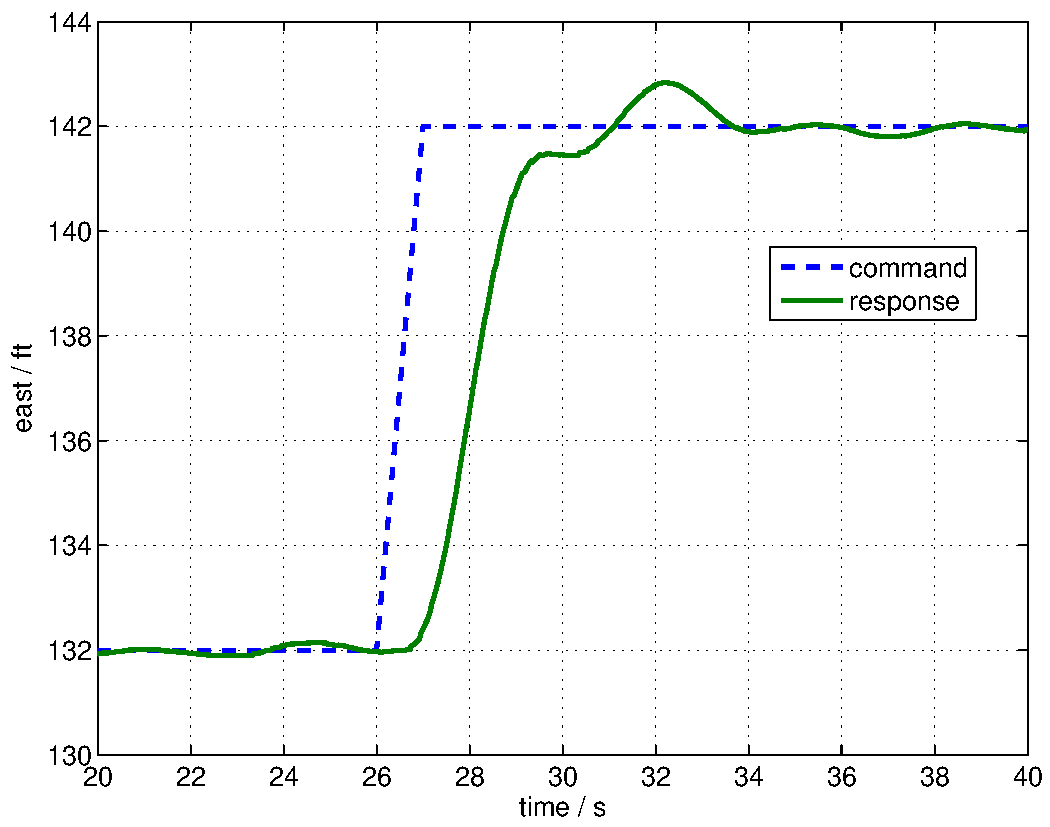
\includegraphics[height=\myfigheight]{ewStep}
  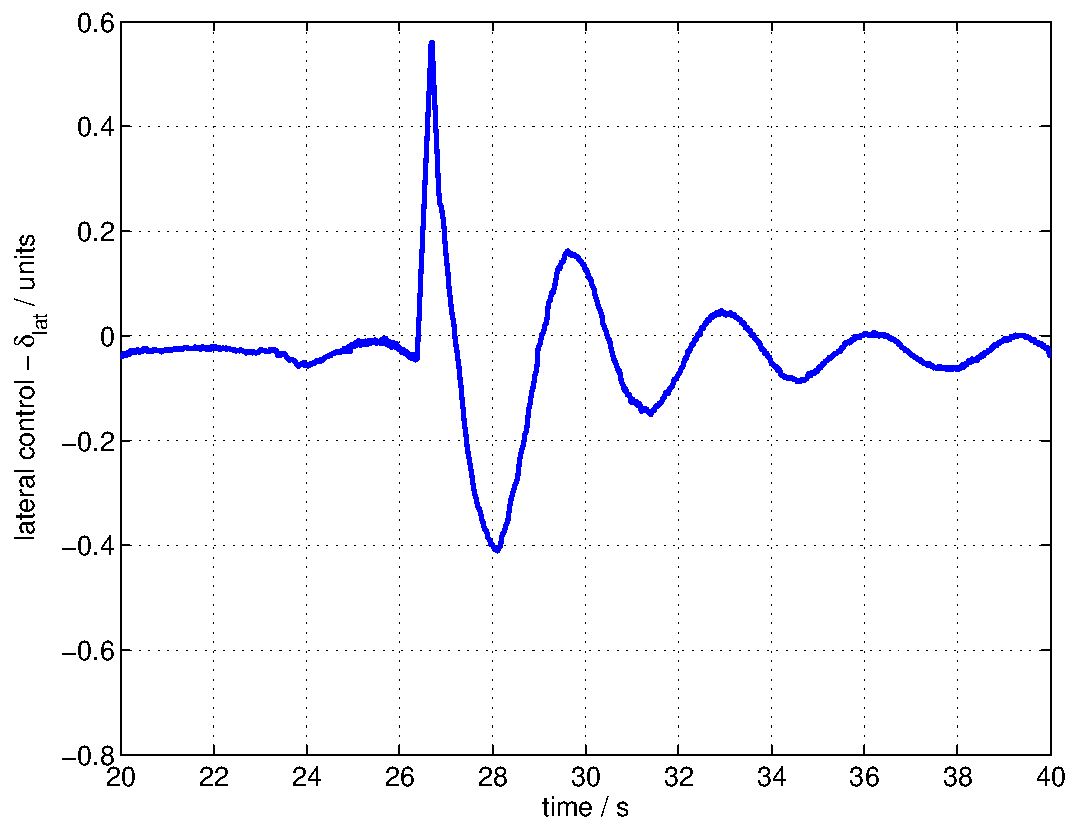
\includegraphics[height=\myfigheight]{ewStepLat}
  \caption{Response to a $20 ft$ step in the lateral direction.}
  \label{f:ewStep}
  \end{center}
\end{figure}
%
\begin{figure}
  \begin{center}
  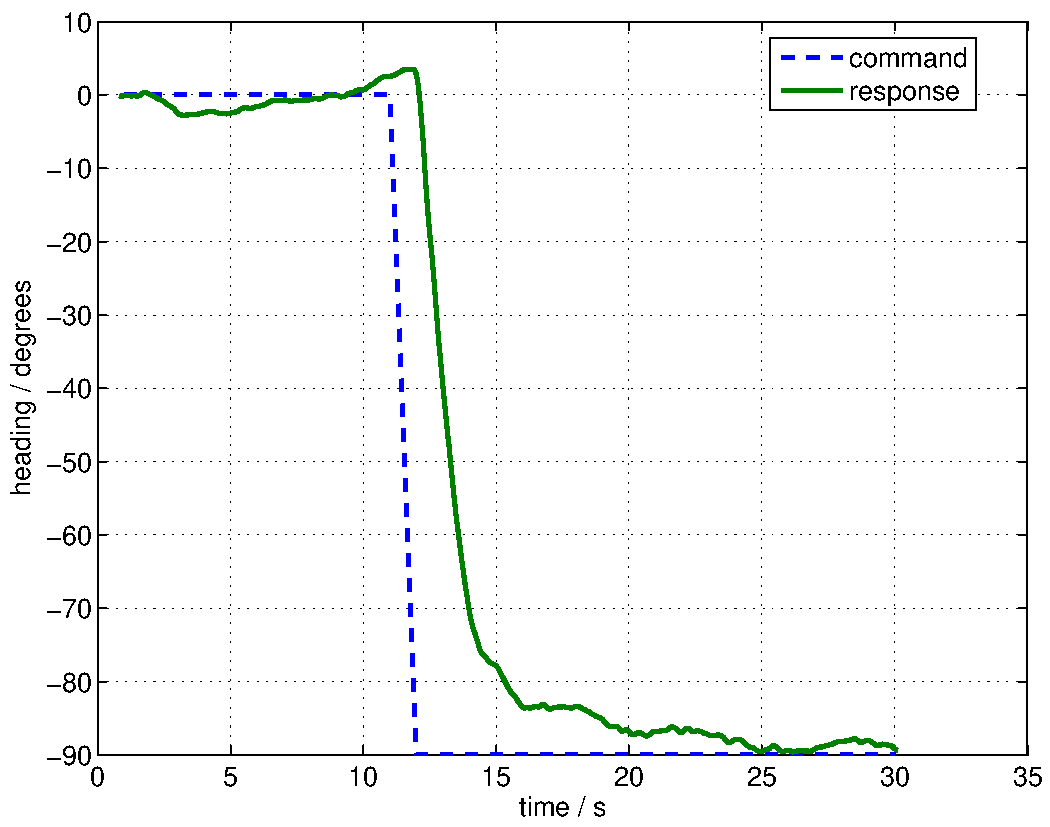
\includegraphics[height=\myfigheight]{headingStep}
  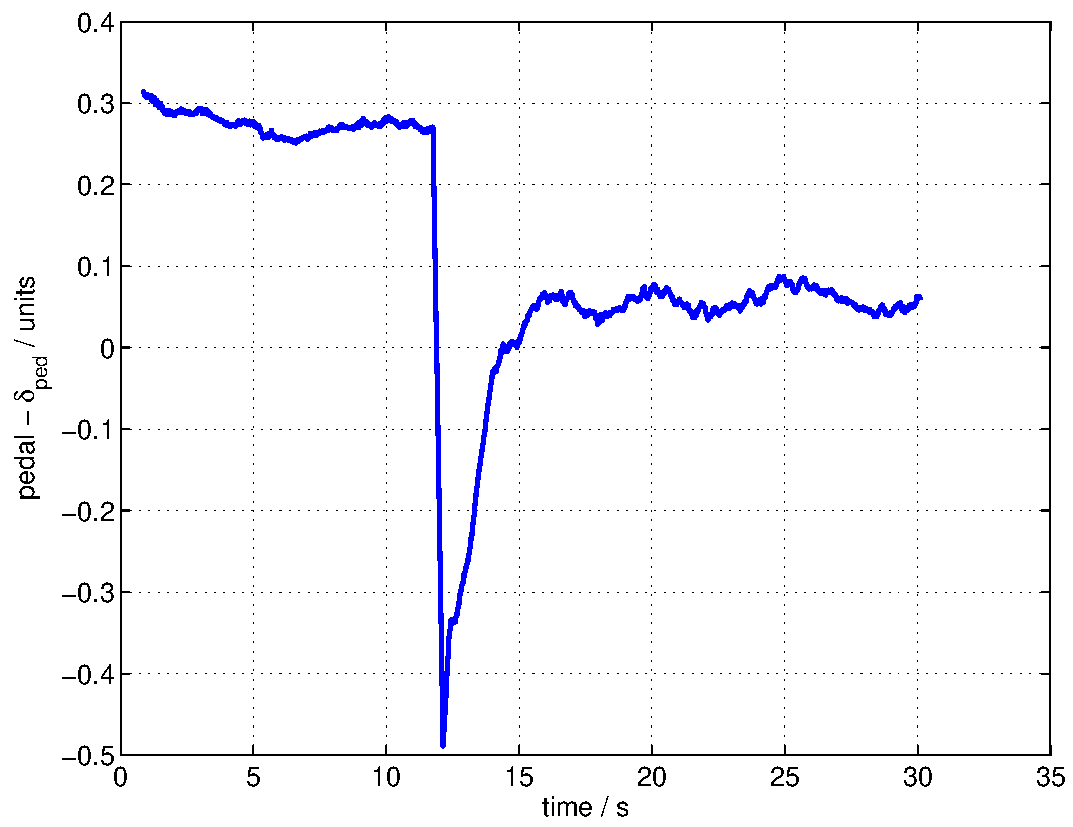
\includegraphics[height=\myfigheight]{headingStepPed}
  \caption{Response to a 90 degree heading command.}
  \label{f:headingStep}
  \end{center}
\end{figure}
Finally, the controller was flight tested on the GTMax helicopter
shown in \fig{f:helipic}. A lateral position step response is shown
in \fig{f:ewStep}.  The vehicle heading was regulated due-north
during this maneuver. Lateral control deflections during the
maneuver were recorded and are also shown. A step heading command
response and pedal control history is shown in \fig{f:headingStep}. It should be noted that during
flight tests, states were sampled at varying rates in order to
conserve memory and datalink bandwidth. The trajectory commands
$\pc,\vc,\qc,\oc$ were sampled at $1 Hz$, actuator deflections
$\delta_{coll},\delta_{lon},\delta_{lat}$ and $\delta_{ped}$ were
sampled at $50 Hz$, vehicle position and speed was sampled at $50
Hz$. Since the command vector is sampled at a low rate ($1 Hz$), a
step command appears as a fast ramp in figures.

\begin{figure}
  \begin{center}
  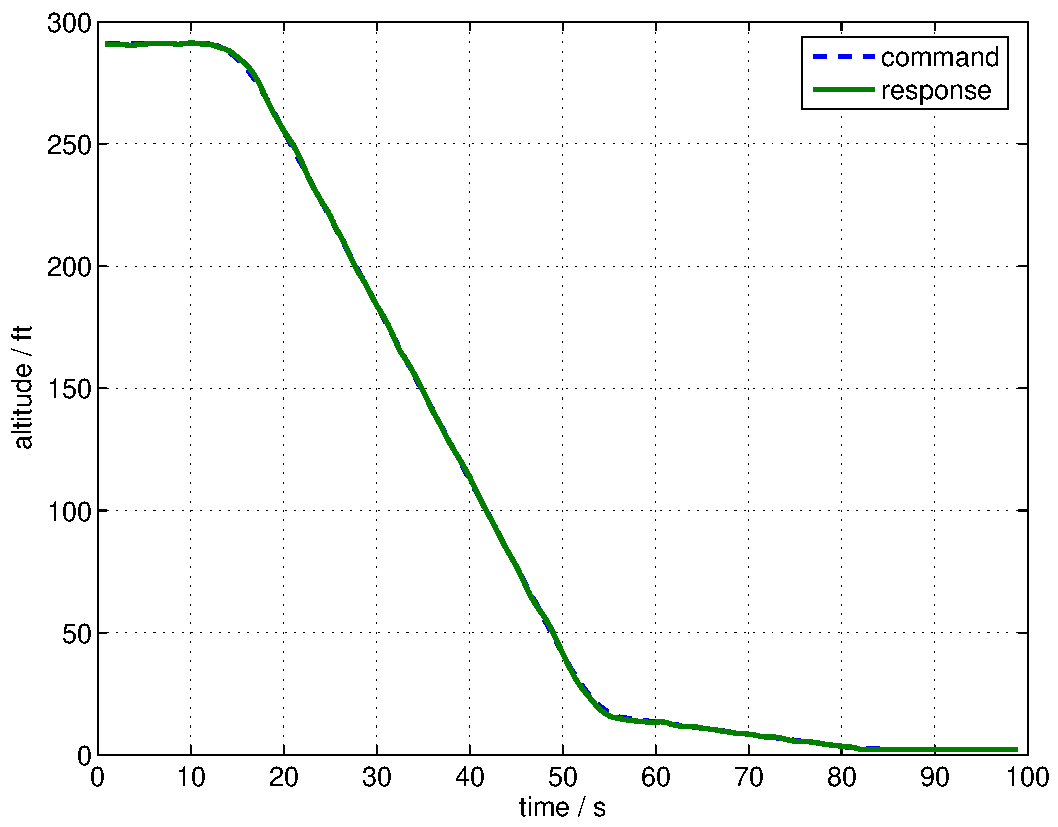
\includegraphics[height=\myfigheight]{landingAlt}
  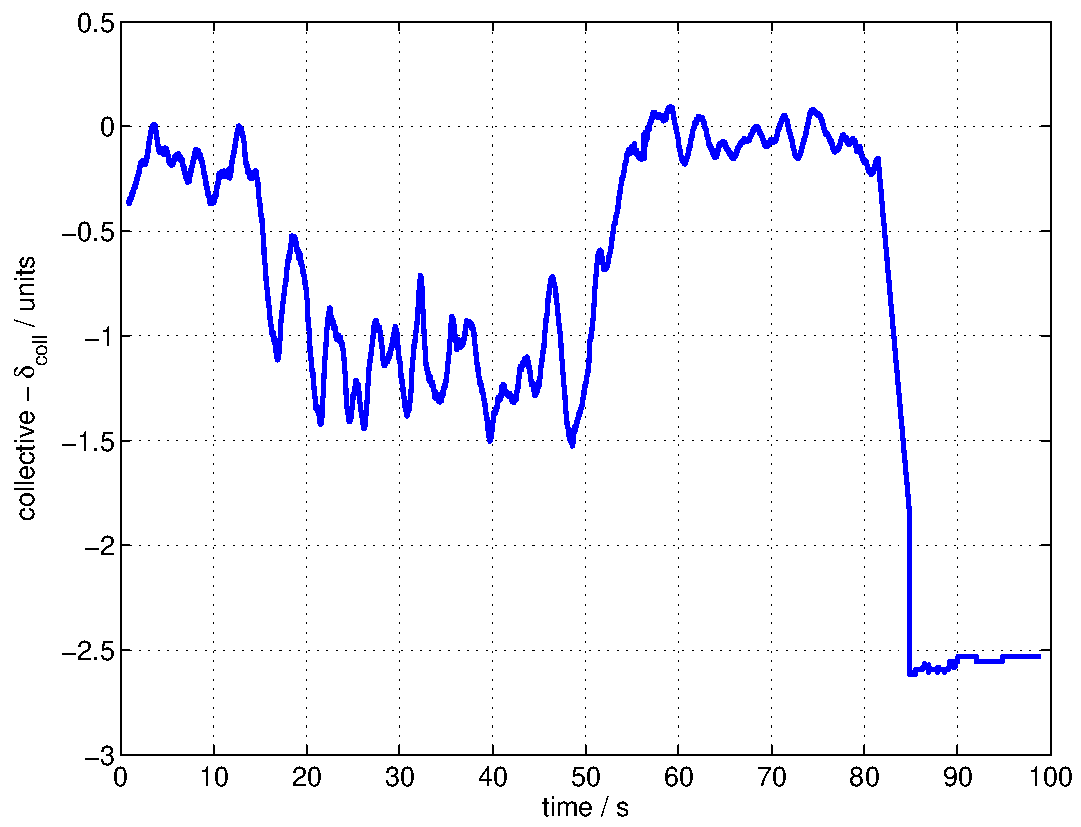
\includegraphics[height=\myfigheight]{landingColl}
  \caption{Automatic landing maneuver.}
  \label{f:landing}
  \end{center}
\end{figure}
%
\begin{figure}
  \begin{center}
  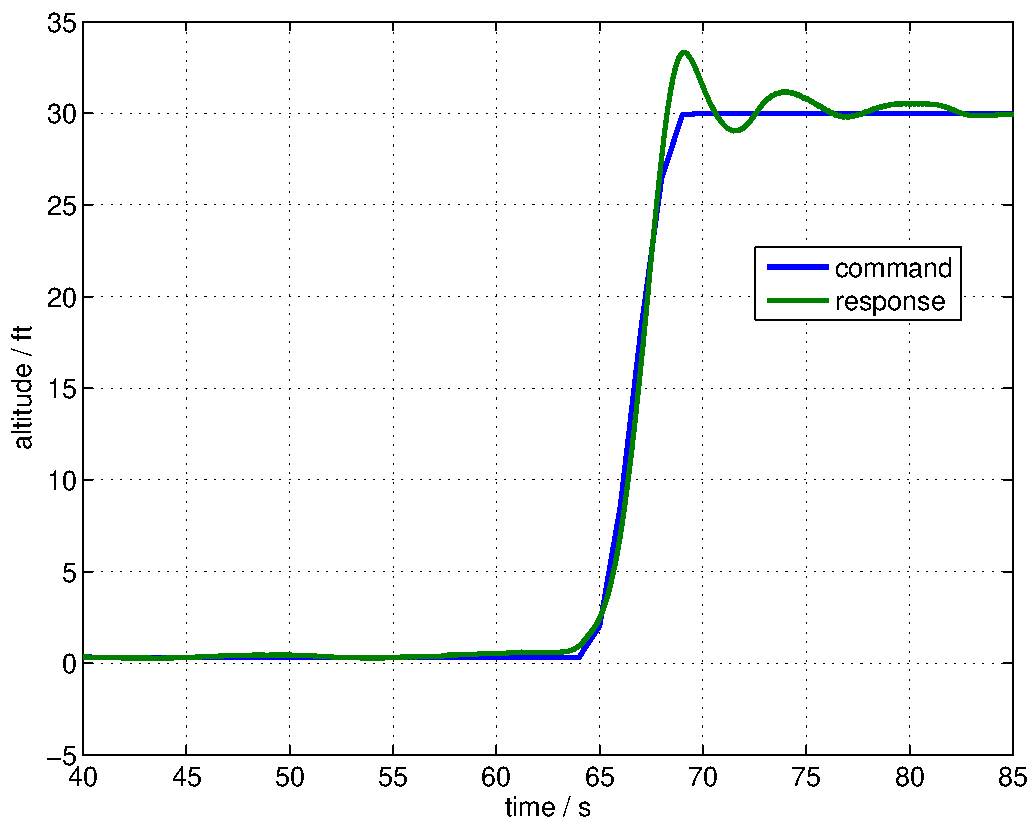
\includegraphics[height=\myfigheight]{takeoffAlt}
  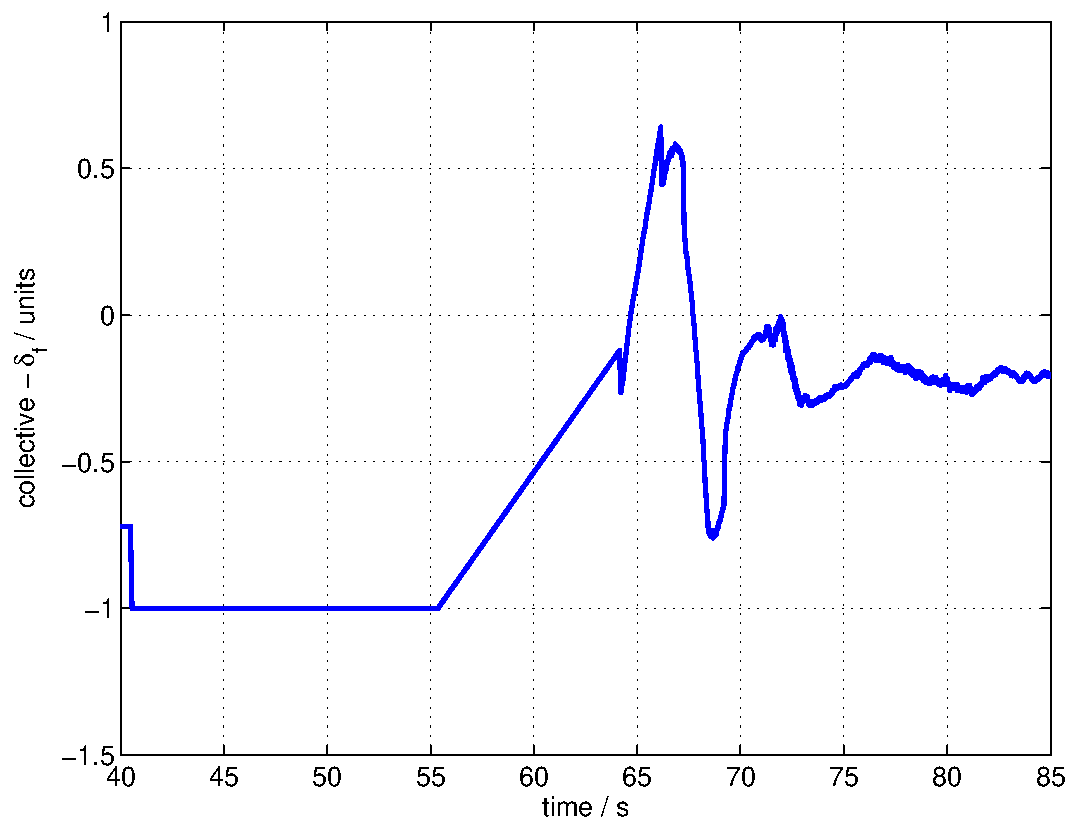
\includegraphics[height=\myfigheight]{takeoffColl}
  \caption{Automatic take-off maneuver.}
  \label{f:takeoff}
  \end{center}
\end{figure}

During takeoff and landing phases a range sensor (sonar) is used to
maintain and update the estimated local terrain altitude in the
navigation system. The sonar is valid up to $8 ft$ above the
terrain, sufficient for landing and takeoff purposes.
\fig{f:landing} illustrates the altitude and collective profile
during a landing. The vehicle starts at an initial hover at $300
ft$, followed by a descent at $7 ft/s$ until the vehicle is $15 ft$
above the estimated terrain. The vehicle then descends at $0.5 ft/s$
until weight-on-skids is automatically detected at which point the
collective is slowly ramped down. Automatic takeoff
(\fig{f:takeoff}) is similar where the collective is slowly ramped
up until weight-on-skids is no longer detected. It should be noted
that NN adaptation is active at all times except when
weight-on-skids is active. Additionally, when weight is on skids,
the collective ramp-up during takeoff and ramp-down during landing
is open-loop.


\begin{figure}
  \begin{center}
%  \subfigure[\label{f:highspeedPos}]{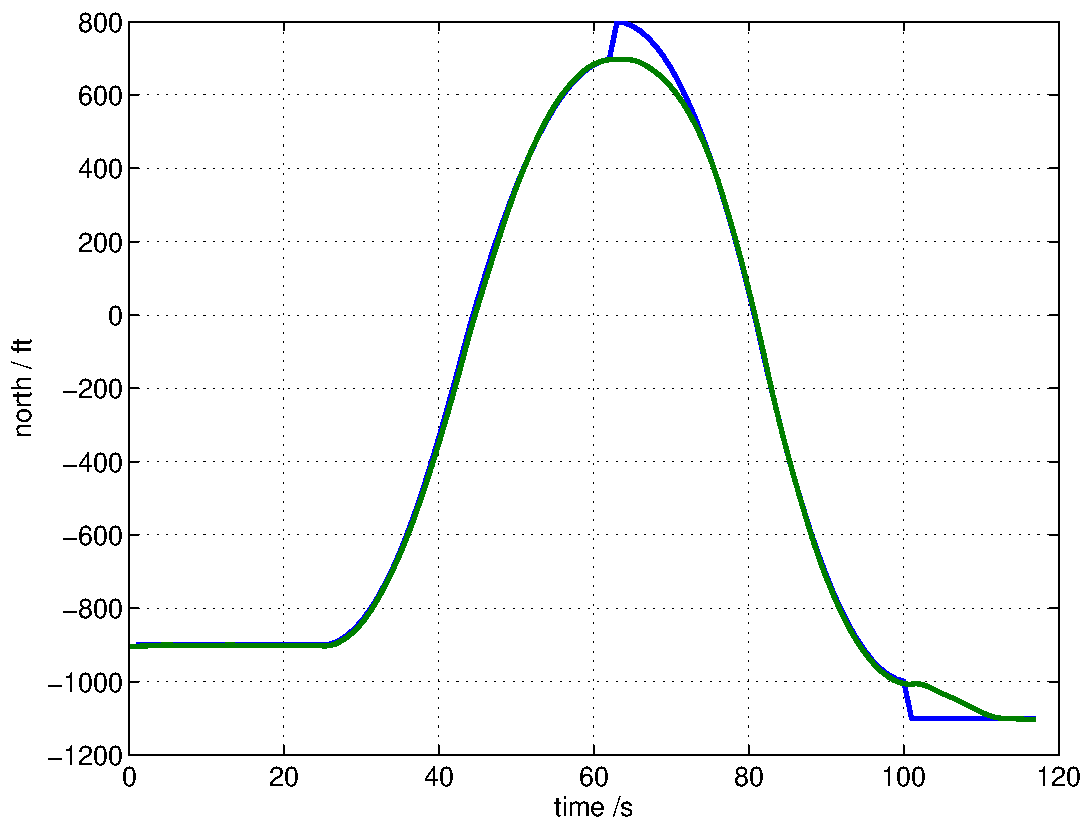
\includegraphics[height=\myfigheight]{highspeedPos}}
  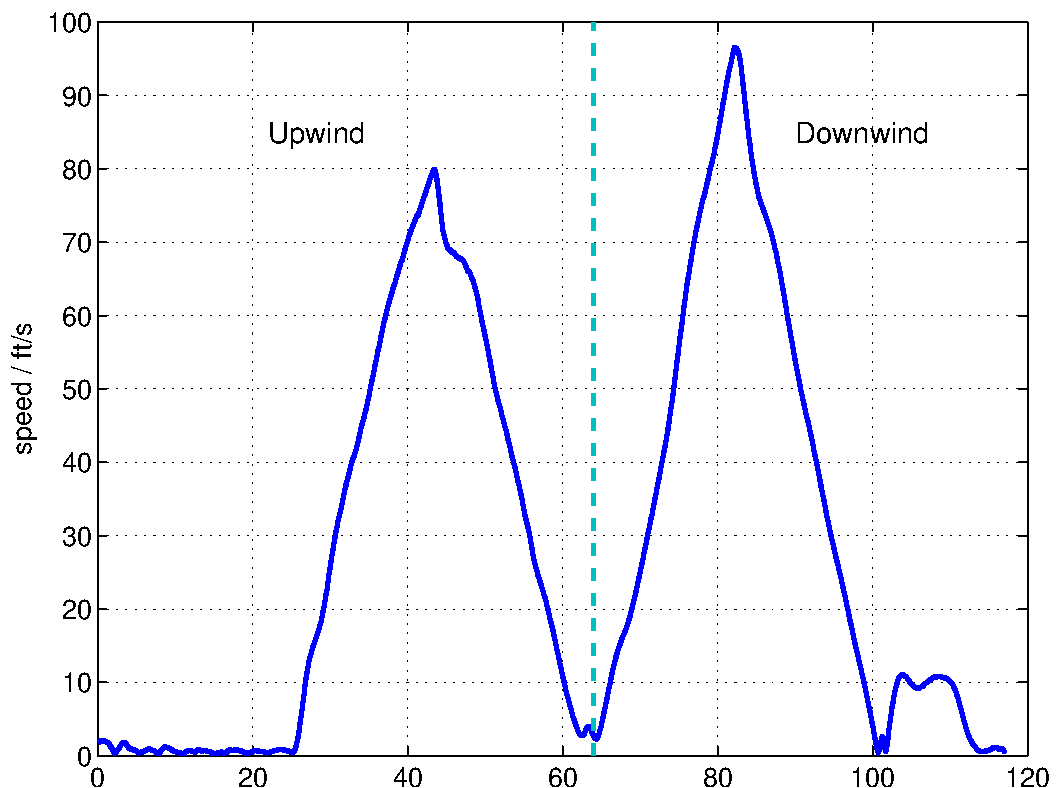
\includegraphics[height=\mytfigheight]{highspeedSpeed}
  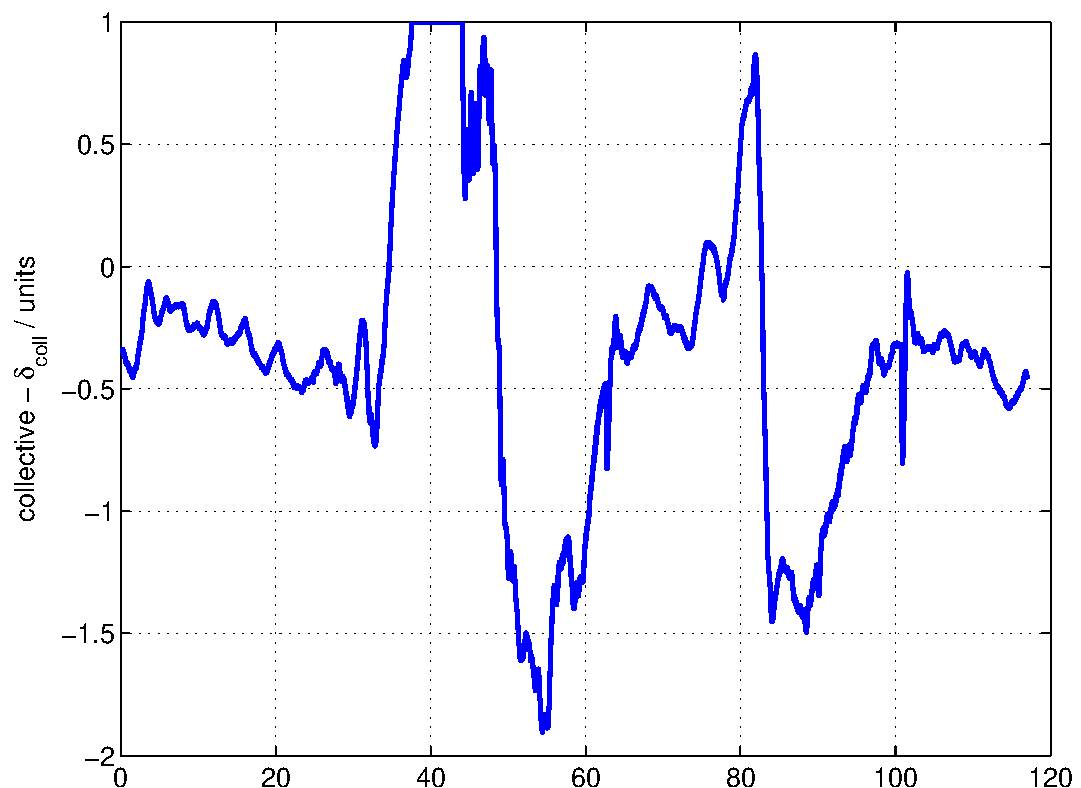
\includegraphics[height=\mytfigheight]{highspeedColl}
  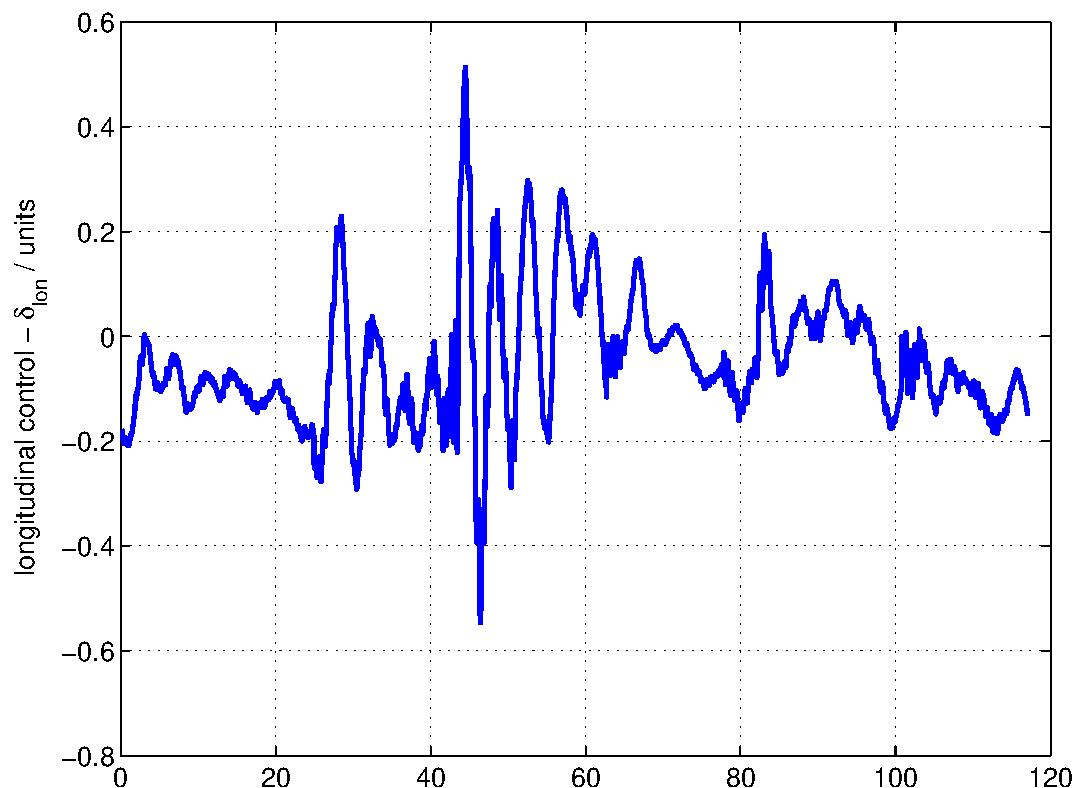
\includegraphics[height=\mytfigheight]{highspeedLong}
  \caption{High speed forward flight up to $97 ft/s$.}
  \label{f:highspeed}
  \end{center}
\end{figure}
\begin{figure}
  \begin{center}
  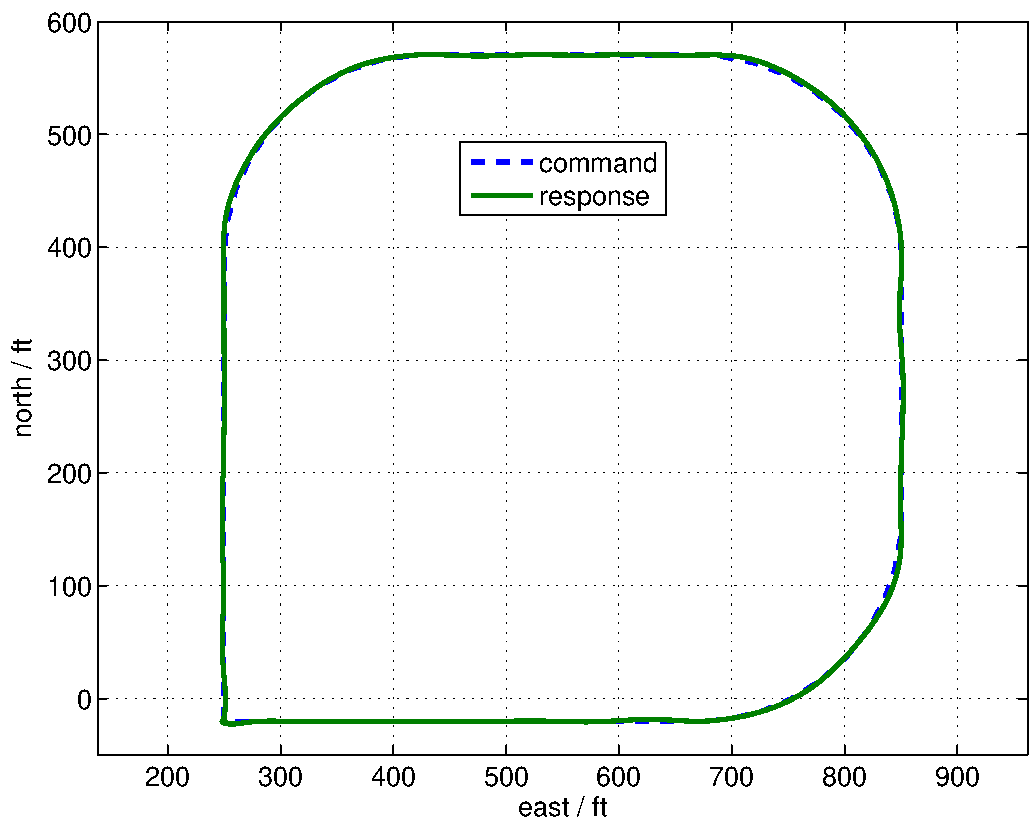
\includegraphics[height=\myfigheight]{squareNorthEast}
  \caption{Flying a square pattern at $30 ft/s$.}
  \label{f:squareNorthEast}
  \end{center}
\end{figure}
\begin{figure}
  \begin{center}
  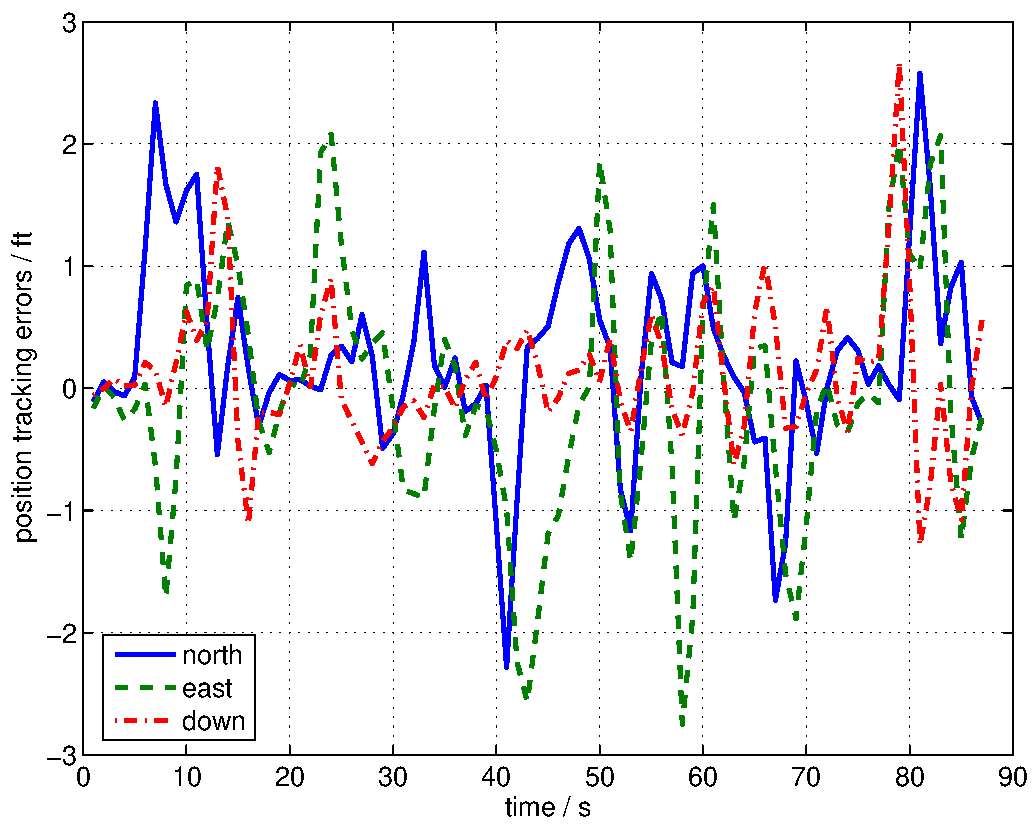
\includegraphics[height=\myfigheight]{squarePosError}
  \caption{Command tracking errors while flying a square pattern at $30 ft/s$.}
  \label{f:squarePosError}
  \end{center}
\end{figure}

The approximate model used to compute the dynamic inverse
(\eq{e:transinverse} and \eq{e:attinverse}) is based on a linear
model of the dynamics in hover. To evaluate controller performance
at different points of the envelope, the vehicle was commanded to
track a trajectory that accelerated up to a speed of $100 ft/s$. To
account for wind, an upwind and downwind leg were flown. In the
upwind leg the vehicle accelerated up to $80 ft/s$ and during the
downwind leg the vehicle accelerated up to a speed of $97 ft/s$ as
shown in \fig{f:highspeed}. Collective and longitudinal control
deflections are also shown. In the upwind leg, the collective is
saturated and the vehicle is unable to accelerate further. The
longitudinal control deflections behave nominally as the vehicle
accelerates and decelerates through a wide range of the envelope.
The NN is able to adapt to rapidly changing flight conditions, from
the baseline inverting design at hover through to the maximum speed
of the aircraft. A conventional proportional-integral-derivative
design would have required scheduling of gains throughout the speed
range. More significantly, classical design would require accurate
models at each point, unlike this design which does not. In addition
to flight at high speeds, tracking performance was evaluated at
moderate speeds, where a square pattern was flown at $30 ft/s$ for
which position tracking is shown in \fig{f:squareNorthEast}.
External command position tracking errors are shown in
\fig{f:squarePosError} with a peak total position error $3.3 ft$ and
standard deviation of $0.8 ft$.

\begin{figure}
  \begin{center}
  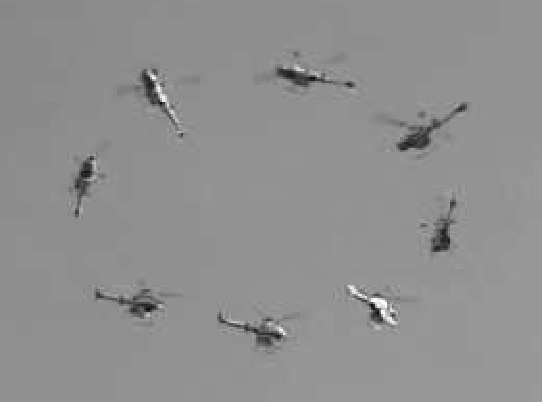
\includegraphics[height=\myfigheight]{pir15m1}
  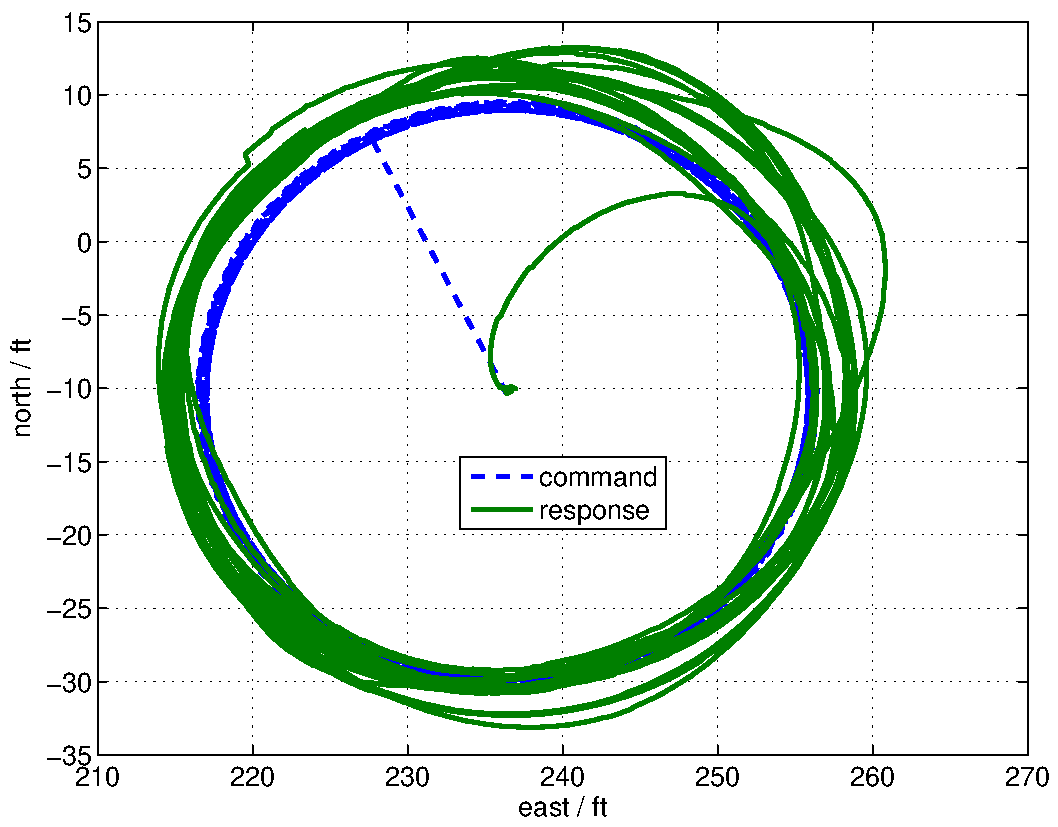
\includegraphics[height=\myfigheight]{pir}
  \caption{Circular maneuver, with 360\textdegree\ heading changes during the circuit.}
  \label{f:pirPosition}
  \end{center}
\end{figure}

\begin{figure}
  \begin{center}
  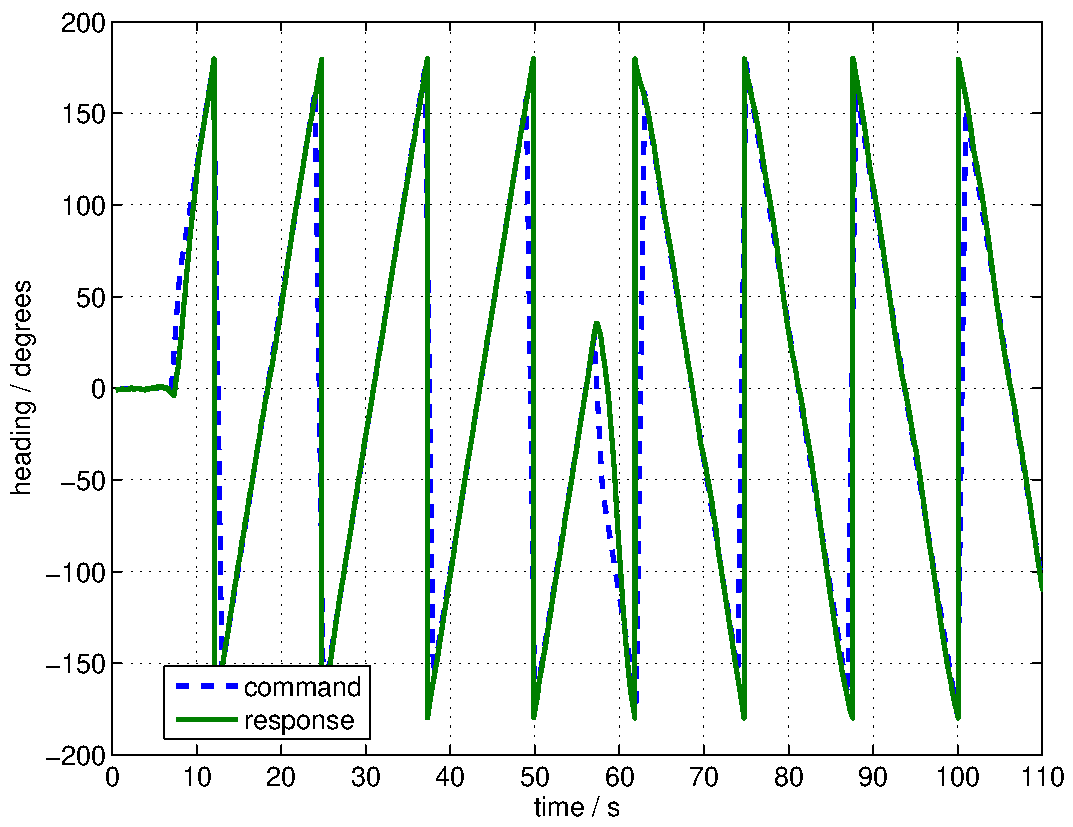
\includegraphics[height=\myfigheight]{pirHeading}
  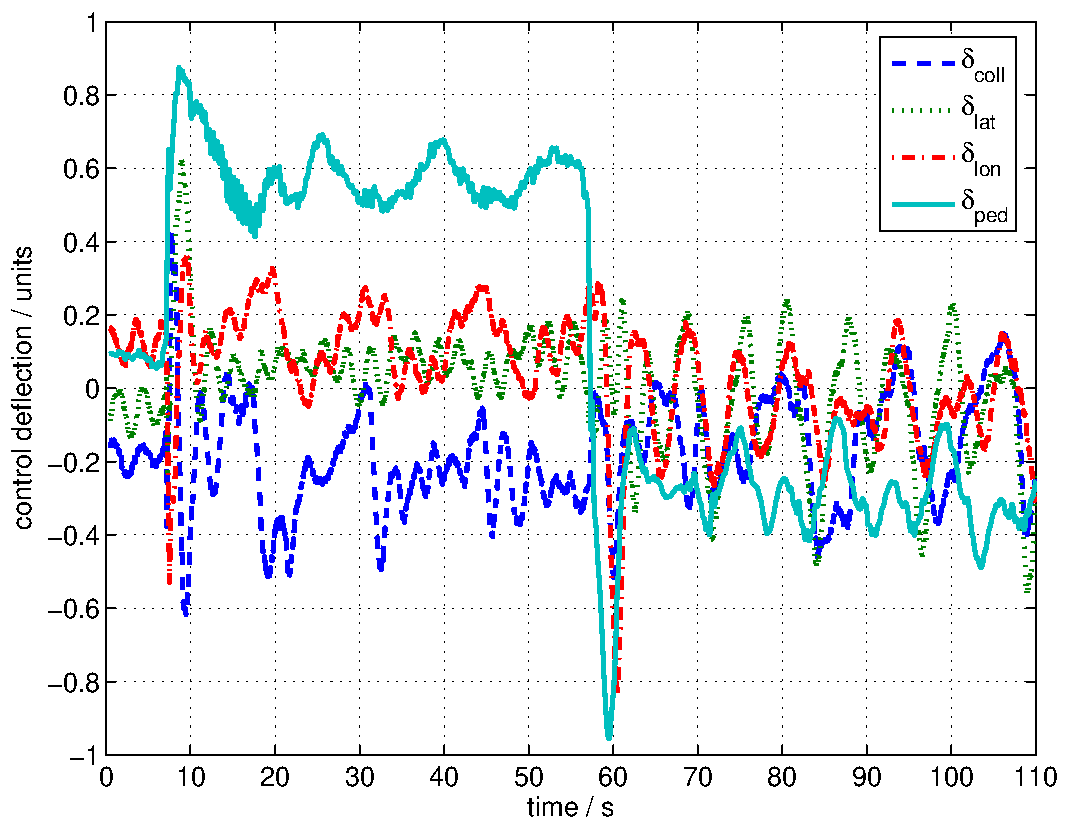
\includegraphics[height=\myfigheight]{pirControls}
  \caption{Heading tracking during circular maneuver and control time history.}
  \label{f:pirHeading}
  \end{center}
\end{figure}

Many maneuvers such as high-speed flight are quasi steady, in the
sense that once in the maneuver, control deflection changes are only
necessary for disturbance rejection. To evaluate performance where
the controls have to vary significantly in order to track the
commanded trajectory, the helicopter was commanded to perform a
circular maneuver in the north-east plane with constant altitude and
a constantly changing heading. The trajectory equations for this
maneuver are given by
\begin{alignat*}{2}
\pc &=
\begin{bmatrix}
\frac{V}{\omega}\cos(\omega t) \\
\frac{V}{\omega}\sin(\omega t) \\
-h
\end{bmatrix},
\qquad \vc &=
\begin{bmatrix}
-V\sin(\omega t) \\
V\cos(\omega t) \\
0
\end{bmatrix}, \nonumber \\
\psi_c &= \omega t f,
\end{alignat*}
where, $t$ is current time and $h$ is a constant altitude command.
$V$ is speed of the maneuver, $\omega$ is angular speed of the
helicopter around the maneuver origin, and $f$ is number of
360\textdegree\ changes in heading to be performed per circuit. If
$\omega=\pi/2 rad/s$, the helicopter will complete the circular
circuit once every 4 seconds. If $f = 1$, the helicopter will rotate
anticlockwise 360\textdegree\ once per circuit. \fig{f:pirPosition}
shows the response to such a trajectory with parameters $\omega =
0.5 rad/s$, $f = 1$, $V = 10 ft/s$. After the initial transition
into the circular maneuver, the tracking is seen to be within 5 ft.
To visualize the maneuver easily, superimposed still images of the
vehicle during the circular maneuver are shown. Both anticlockwise
and clockwise heading changes during the maneuver were tested by
changing the parameter from $f=1$ (anticlockwise) to $f = -1$
(clockwise) at $t = 55s$. \fig{f:pirHeading} shows that heading
tracking is good in both cases. The time history of the pedal input
$\delta_{ped}$ and all other controls during the maneuver is also
shown and illustrates how the vehicle has to exercise all of its
controls during this maneuver.

\begin{figure}
  \begin{center}
  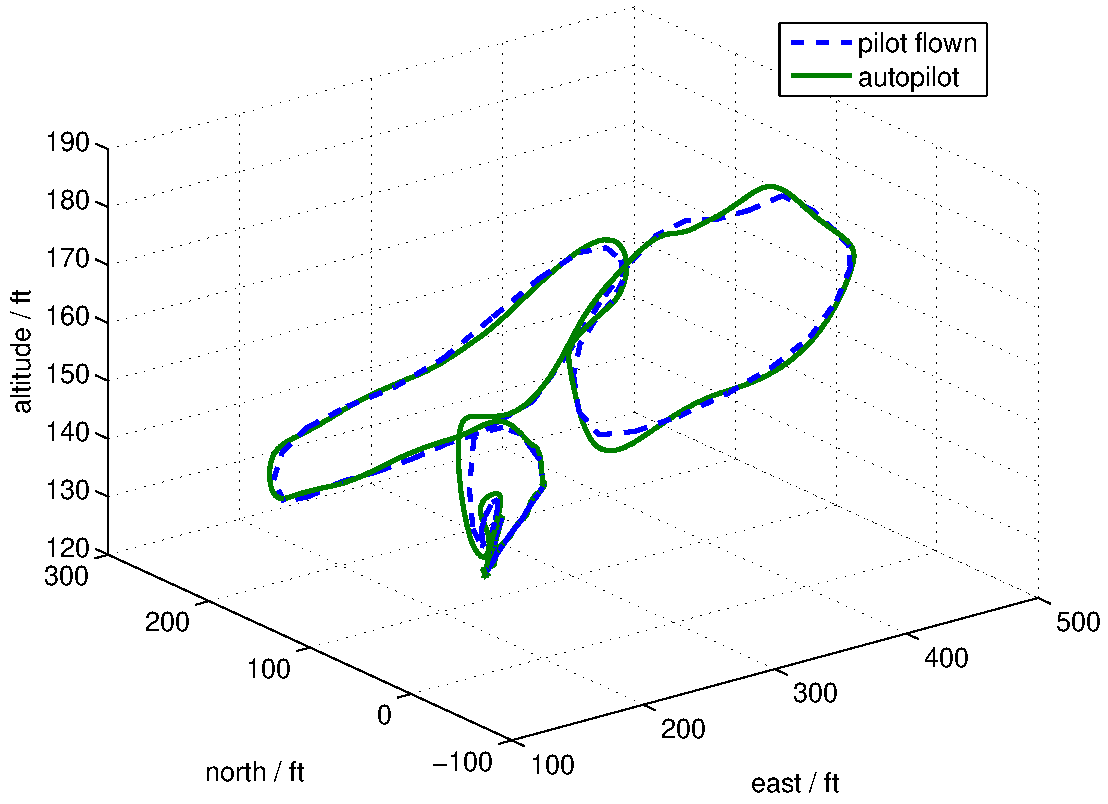
\includegraphics[height=\myfigheight]{pilottrack3d}
  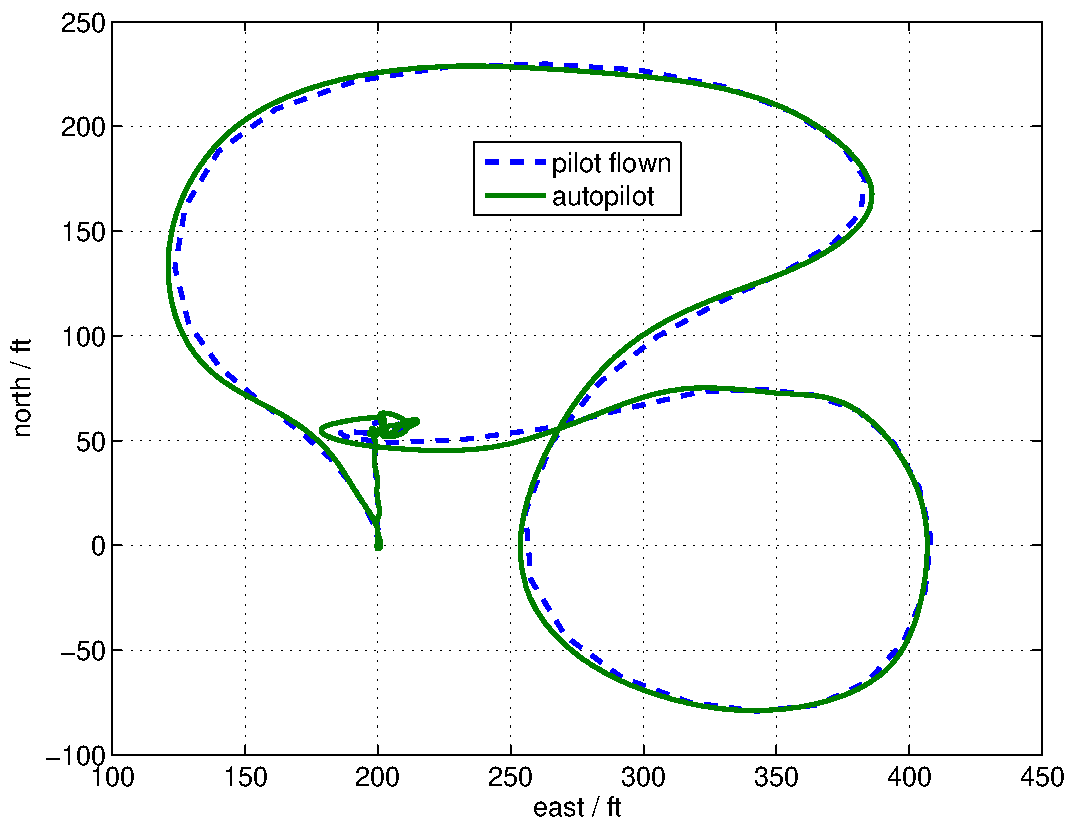
\includegraphics[height=\myfigheight]{pilottrackNorthEast}
  \caption{A 3D view and ground track view, of a trajectory initially flown manually by a pilot and then tracked by the controller.}
  \label{f:pilottrack3d}
  \end{center}
\end{figure}


Next, the ability of the controller to track a previous
manually-flown maneuver was tested. First, a human pilot flew a
figure eight, 3-dimensional pattern with the vehicle. Vehicle state
was recorded and was then played back as commands to the adaptive
controller. A 3D plot of the pilot and controller flown trajectories
are shown in \fig{f:pilottrack3d} along with projected ground track.
Overall, the tracking in position was measured to be within $11.3
ft$ of the desired pilot flown trajectory with a standard deviation
of $4.7 ft$.
%
%  \subfigure[\label{f:eturnNorthAltitude}]{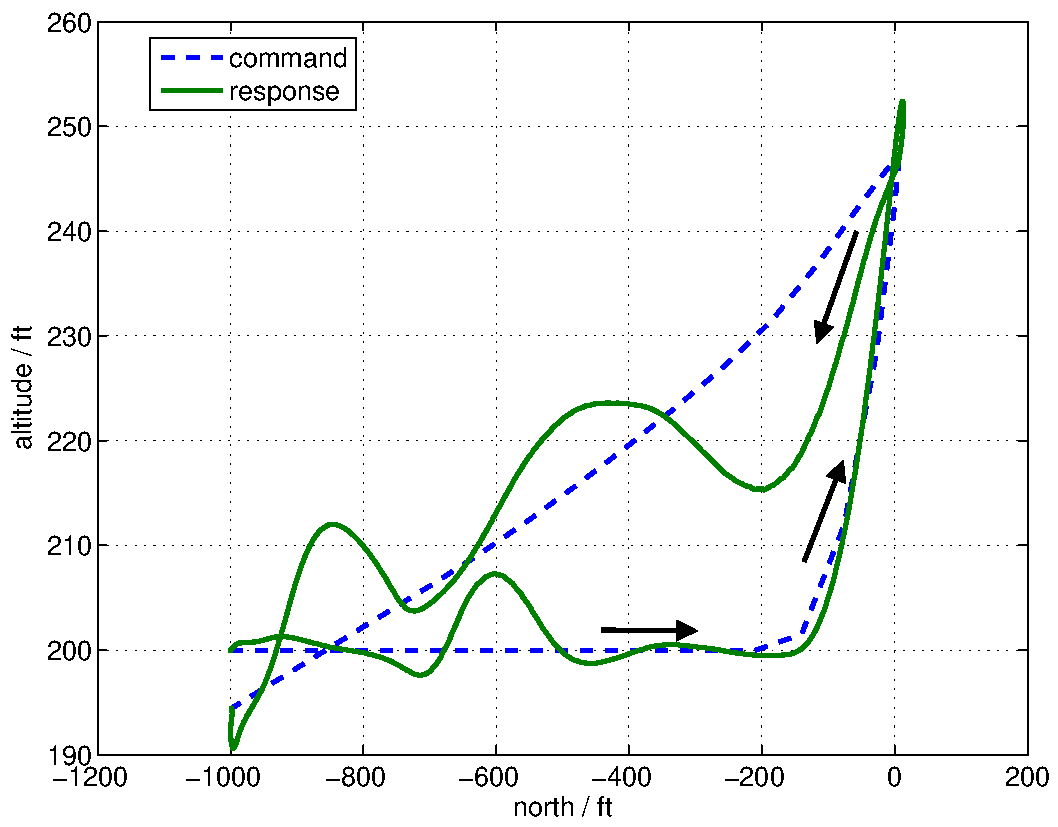
\includegraphics[height=\myfigheight]{eturnNorthAltitude}}
%  \subfigure[\label{f:eturnAlt}]{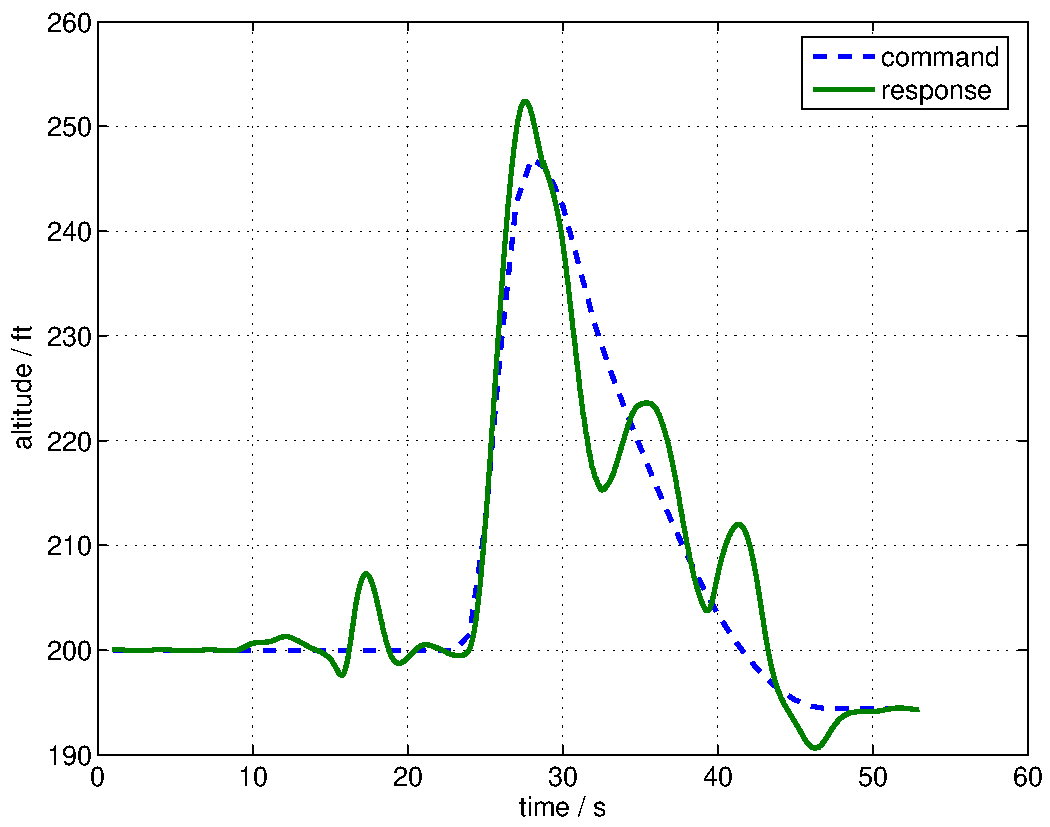
\includegraphics[height=\myfigheight]{eturnAlt}}
%  \subfigure[\label{f:eturnTheta}]{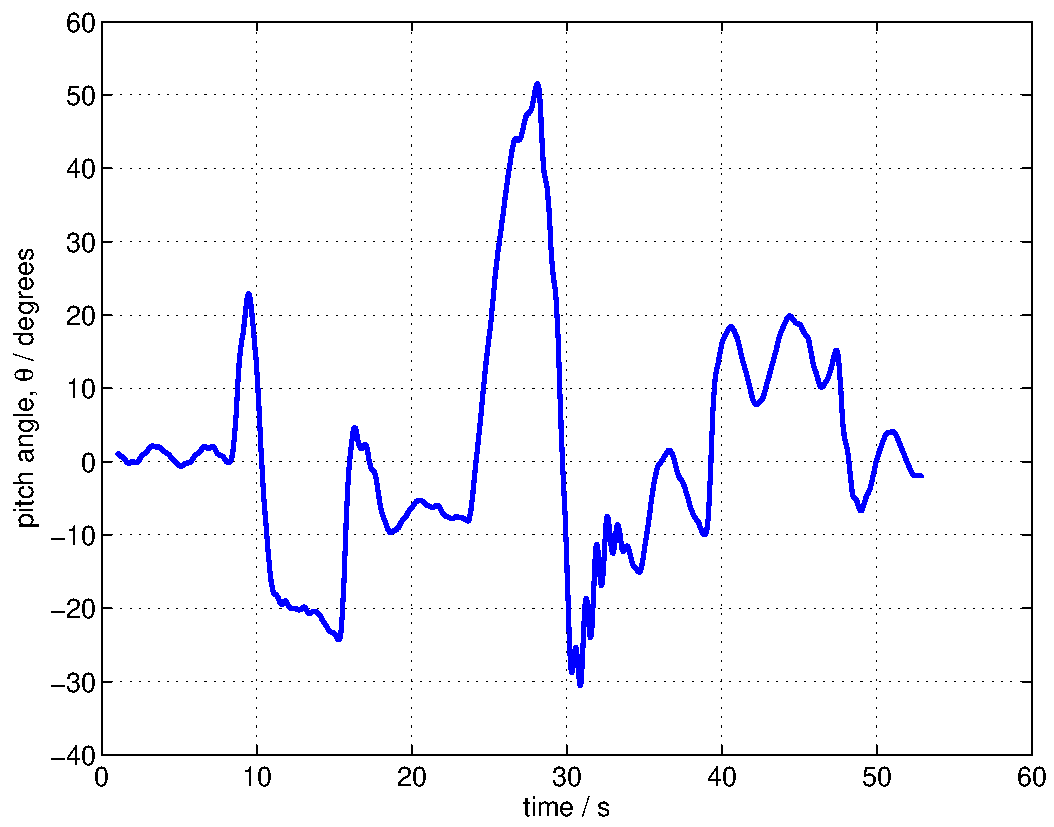
\includegraphics[height=\myfigheight]{eturnTheta}}
%  \subfigure[\label{f:eturnColl}]{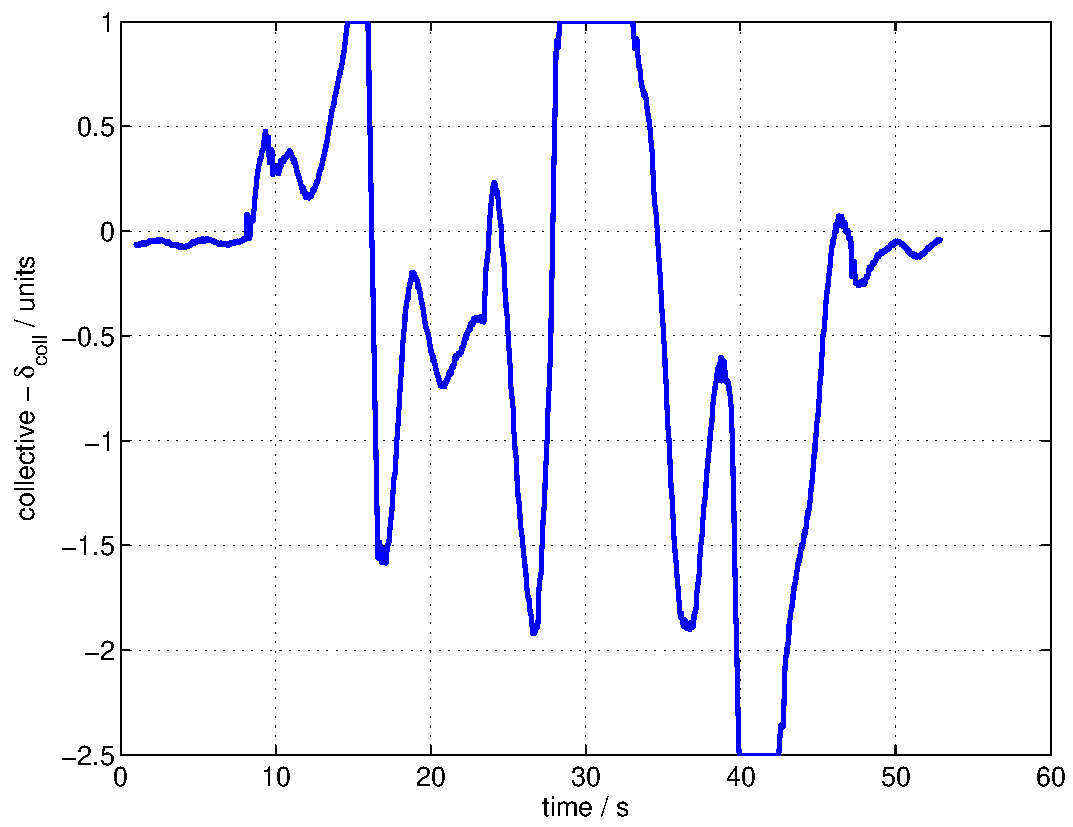
\includegraphics[height=\myfigheight]{eturnColl}}

\begin{figure}
  \begin{center}
  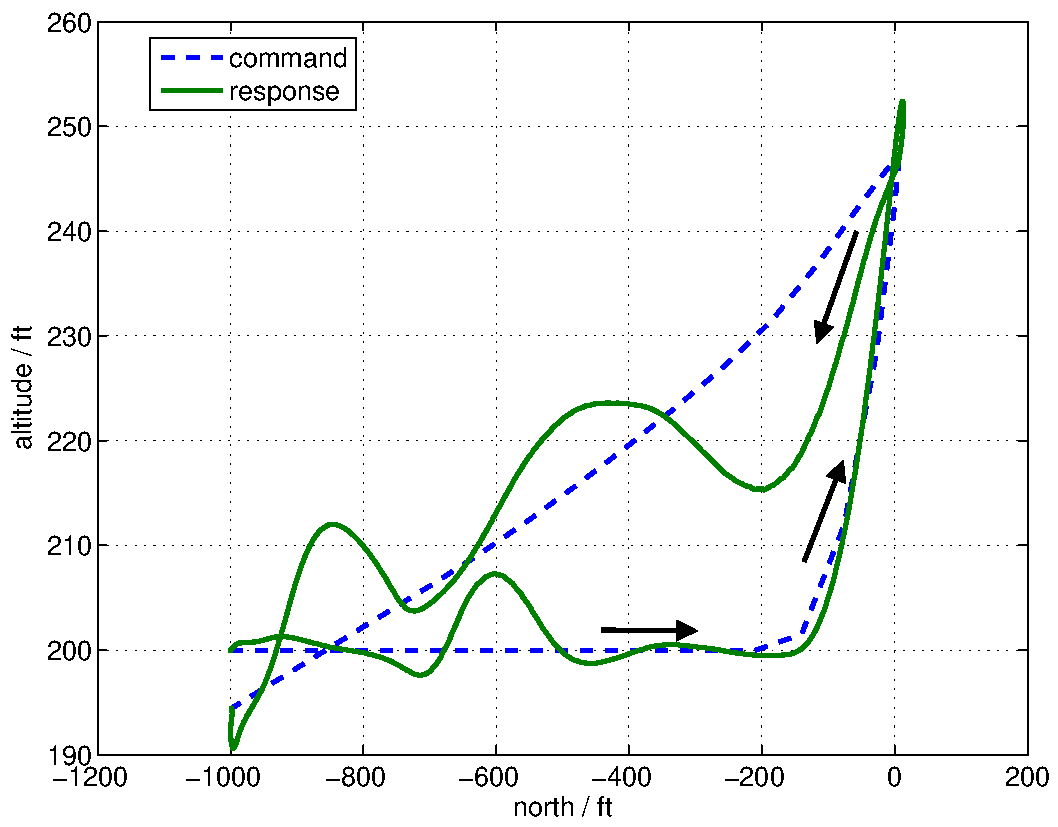
\includegraphics[height=\myfigheight]{eturnNorthAltitude}
  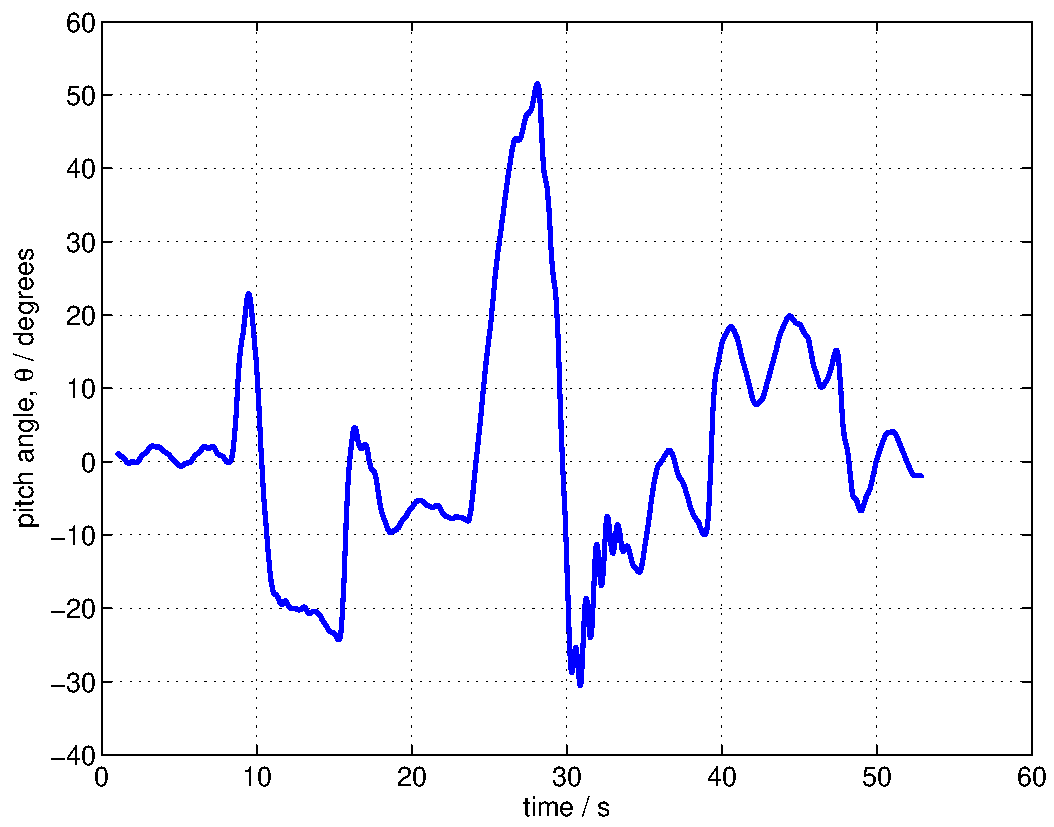
\includegraphics[height=\myfigheight]{eturnTheta}
  \caption{North-Altitude and pitch angle profile during a 180\textdegree\ velocity change maneuver. \emph{Note: North axis and Altitude axis scales are not equal}.}
  \label{f:eturnAltTheta}
  \end{center}
\end{figure}

\begin{figure}
  \begin{center}
  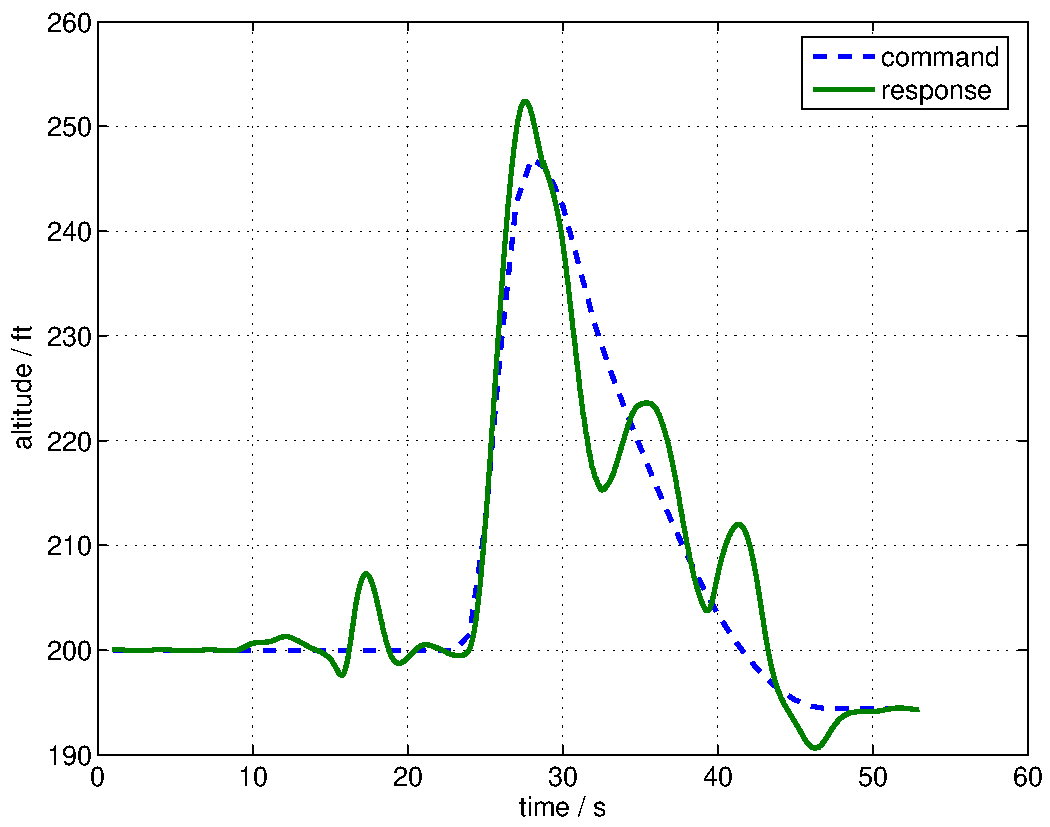
\includegraphics[height=\myfigheight]{eturnAlt}
  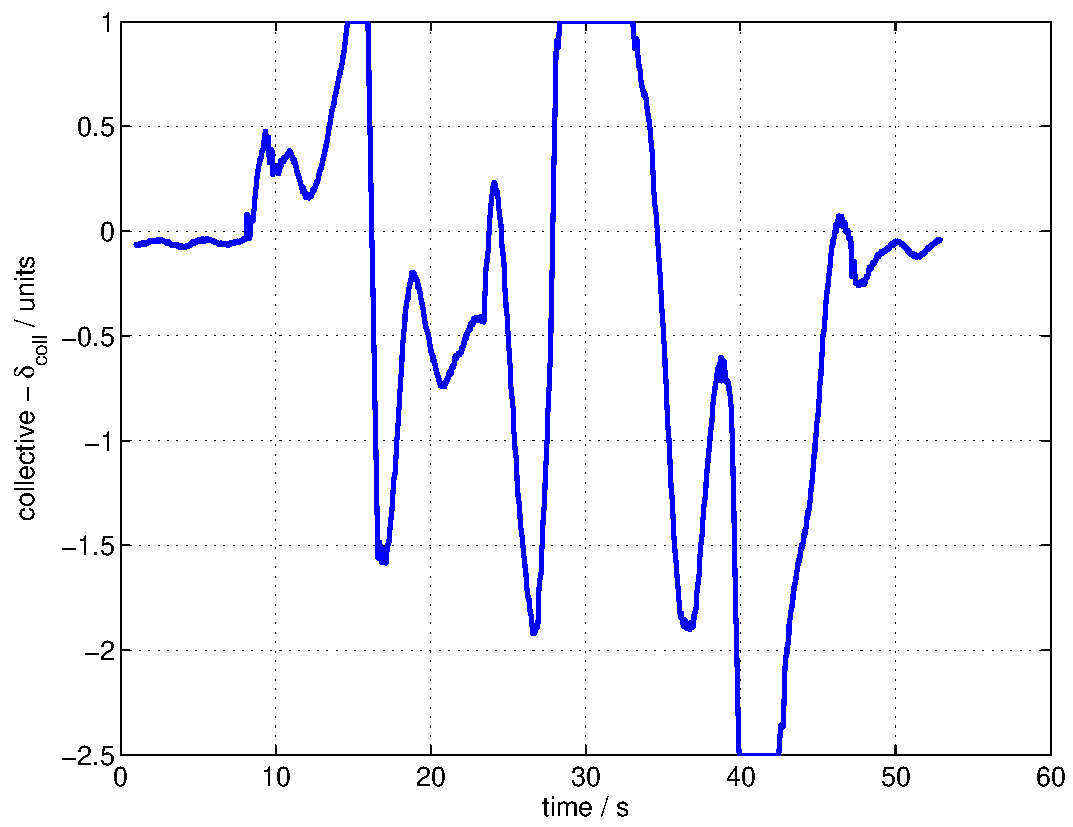
\includegraphics[height=\myfigheight]{eturnColl}
  \caption{Altitude and collective control history during a 180\textdegree\ velocity change maneuver.}
  \label{f:eturnAltColl}
  \end{center}
\end{figure}

Finally, a tactically useful maneuver was flown to test controller
performance at high speeds and pitch attitudes. The objective of the
maneuver is to make a 180-degree velocity change from a forward
flight condition of $70 ft/s$ north to a $70 ft/s$ forward flight
going south. The trajectory command and response in the
north-altitude plane is shown in \fig{f:eturnAltTheta} along with
the pitch angle. A time history of the altitude and the collective
control deflection is shown in \fig{f:eturnAltColl}. During the
maneuver the helicopter is commanded to increase altitude by up to
$50 ft$ in order to minimize saturation of the down collective. In
the deceleration phase the vehicle is able to track the command
trajectory well; however in accelerating to $70 ft/s$ going south,
tracking performance suffers. In both the acceleration and
deceleration phases, poor tracking corresponds with saturation of
the collective control. The oscillations in altitude in
\fig{f:eturnAltColl} are expected and are due to control saturation
which limits the vehicle's descent rate. The large pitch attitudes
experienced are what the outer-loop inversion evaluates as being
required to perform such rapid decelerations and accelerations. This
experiment is an example of maneuvering where the commanded
trajectory is more aggressive than the capability of the vehicle and
is reflected by the extended periods of saturation. It is possible
to operate at the limits of the vehicle primarily due to PCH which
protects the adaptation process.
%
%%%% pirouette
%
%\begin{figure}
%  \begin{center}
%  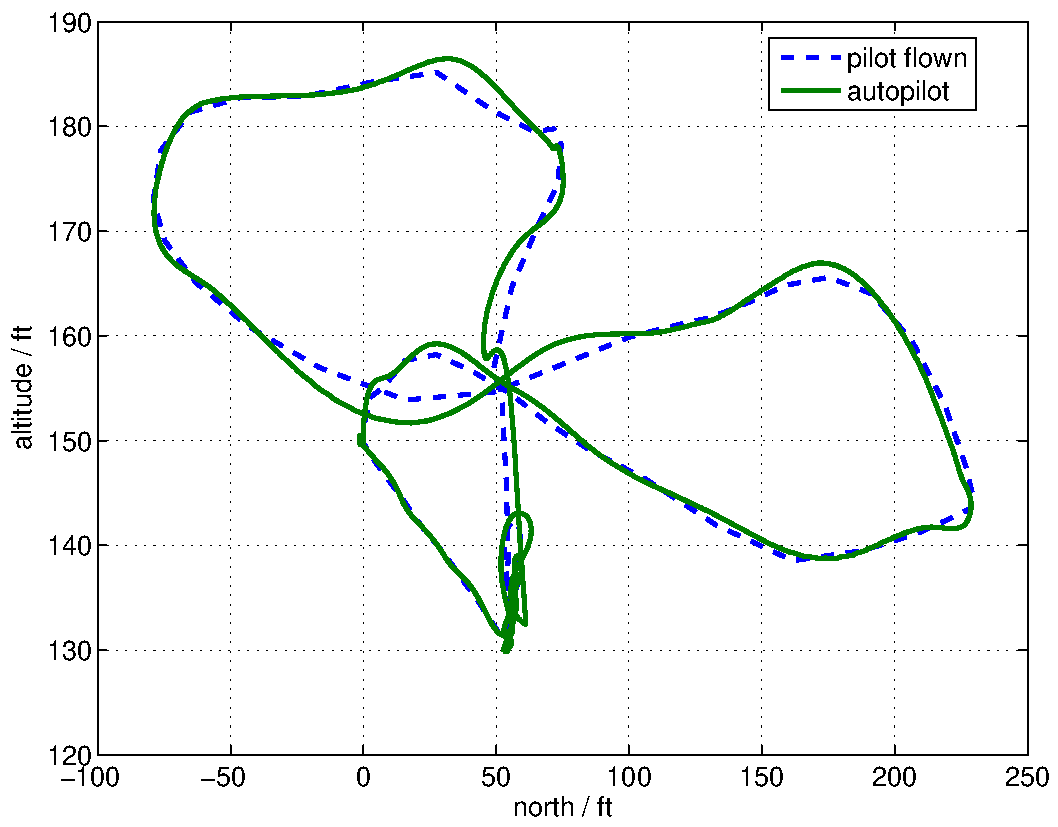
\includegraphics[height=\myfigheight]{pilottrackNorthAltitude}
%  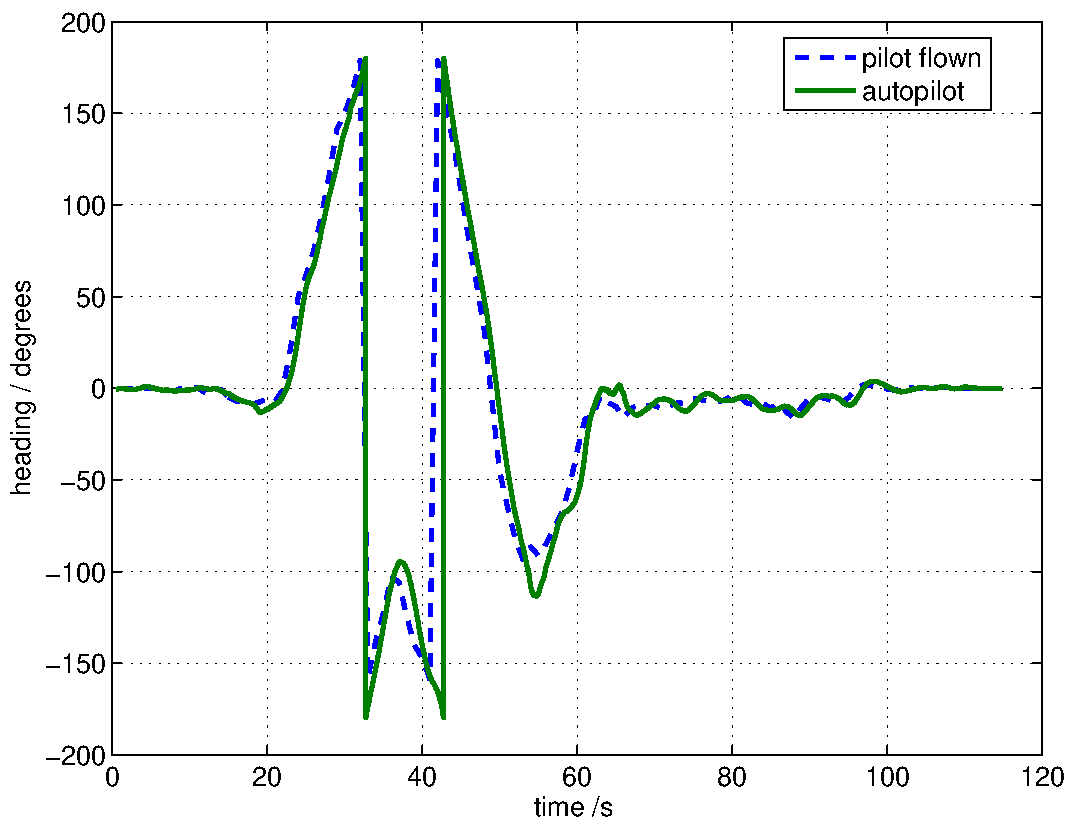
\includegraphics[height=\myfigheight]{pilottrackHeading}
%  \caption{North-Down plane and heading tracking of a trajectory initially flown manually by a pilot and then tracked by the controller.}
%  \label{f:pilottrackAltHead}
%  \end{center}
%\end{figure}
%
\subsection{Application to a Ducted Fan}
\begin{figure}
  \begin{center}
  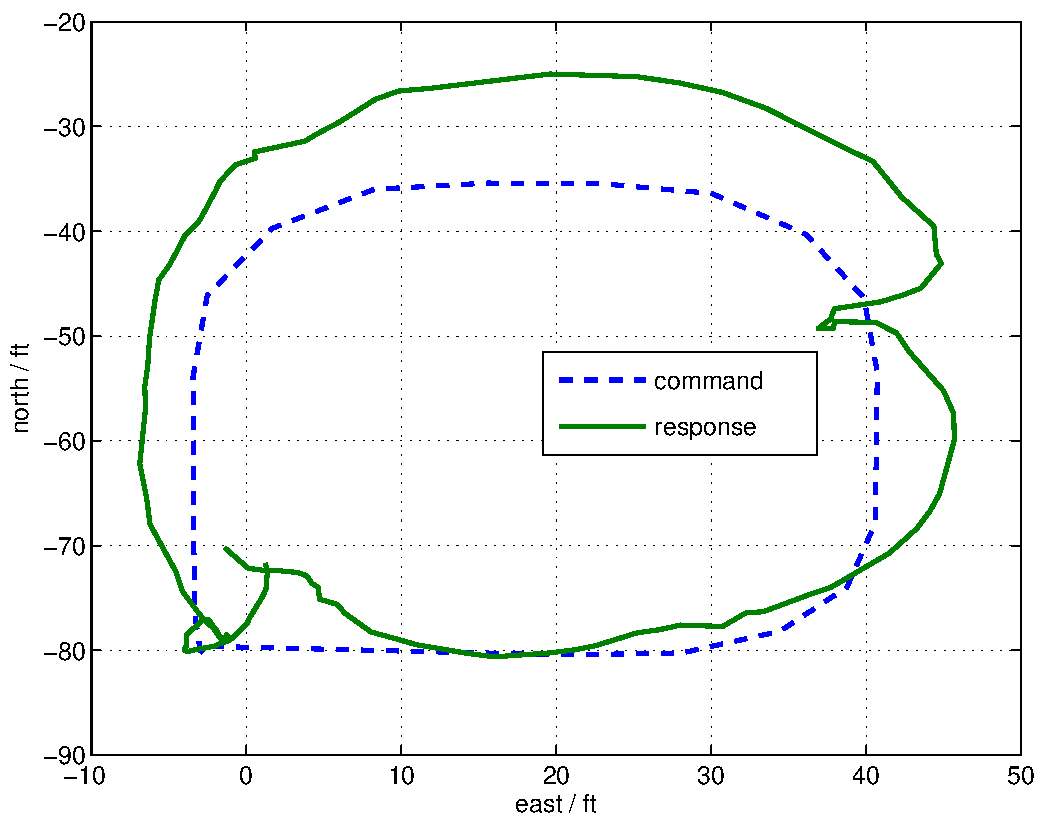
\includegraphics[height=\myfigheight]{gtspyBox2}
  \caption{The GTSpy performing a box maneuver}
  \label{f:gtspyBox}
  \end{center}
\end{figure}
%
\begin{figure}[h]
  \begin{center}
  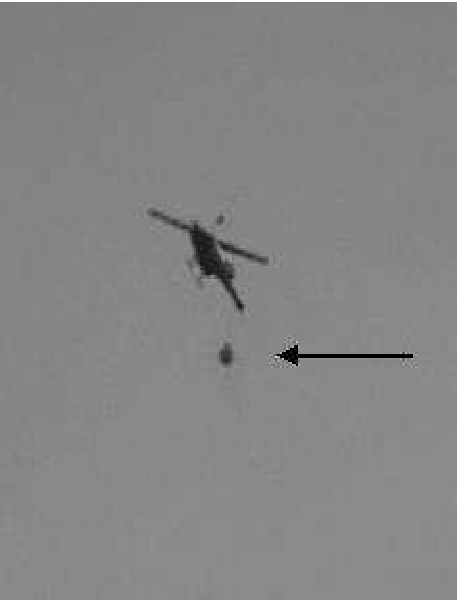
\includegraphics[height=\myfigheight]{gtspyMidAir}
  \caption{Deployment of the GTSpy ducted fan from the GTMax helicopter}
  \label{f:gtspyMidAir}
  \end{center}
\end{figure}
Following tests on the GTMax helicopter, the control method
presented in this chapter was applied to other smaller aircraft. The
algorithms were ported to a custom DSP/FPGA hardware device (the
FCS20) along with a small sensor board that contained gyroscopes and
accelerometers for inertial sensing and a GPS. The avionics package
weighed less than $1 lb$ and fell within the payload capacity of the
11-inch ducted fan (GTSpy). The GTSpy has a maximum take-off weight
of $5.5 lbs$ and is driven by a two-bladed fixed-pitch propeller.
The propeller is enclosed in an annular wing duct with an outer
diameter of $11 inches$. Vanes located directly beneath the
propeller move in order to provide yaw control about the propeller
axis. Two sets of control surfaces located further below the
propeller move in order to provide pitch and roll moments.
Maneuvering is accomplished by tilting the thrust vector with the
control surfaces relying primarily on inflow for dynamic pressure
during hover. Following satisfactory tethered tests, the vehicle was
untethered and allowed to fly simple missions. \fig{f:gtspyBox}
shows a plan view of a small $50\time50 ft$ box maneuver and the
GTSpy's tracking. The large deviation on the eastern side of the box
is most likely due to a wind gust. Another maneuver performed was
the mid-air deployment of the GTSpy. The GTSpy was mounted on the
GTMax helicopter with its engine on and then deployed from a safe
altitude. The GTSpy was able to recover from the initial deployment
transient and maintain attitude and position within 5 seconds of
launch. \fig{f:gtspyMidAir} shows the GTSpy and GTMax during the
deployment transient. Both the GTMax and GTSpy were under computer
control during this maneuver and is the first known deployment of a
rotorcraft from another rotorcraft.
%

%\processdelayedfloats
%
\subsection{Application to a Fixed Wing Aircraft}
The control method presented in this chapter was further applied to a
high-thrust-to-weight ratio fixed wing aircraft with conventional
aircraft controls and a fixed pitch two-bladed propeller. The
dynamic inverse used for control purposes approximated the aircraft
in hover mode where the body axis was defined as
\[
x_{heli} = L_2(-\pi/2)x_{airplane}
\]
where $L_2$ is a rotation matrix around the airplane's body y-axis.
Hence the ailerons control helicopter-yaw, the rudder controls
helicopter-roll and the elevators continue to control pitch. The
external commands provided to the control algorithm contains a
commanded pitch angle as a function of speed. Inner-loop gains were
based on $2.5, 1.5, 2.5 rad/s$ for the (helicopter) roll, pitch and
yaw axis respectively. Outer-loop gains were based on $1.5, 1.0, 0.7
rad/s$ for the x, y and z helicopter-body-axis respectively. The
output-layer learning rates $\Gamma_W$ was set to unity on all
channels and a learning rate of $\Gamma_V$ was set for all inputs.
Reference model parameters were set to $v_{lim} = 10 ft/s$ and
$\omega_{lim} = 1.0 rad/s$. The control effectiveness $B$ was scaled
based on speed in order to reflect the reduced control authority of
the control surfaces in hover. Flight tests were initiated with the
airplane performing circular orbits and gradually lowering airspeed
until hover. The reverse, transition to forward flight was
accomplished by a more aggressive command into forward flight.
\begin{figure}
  \begin{center}
  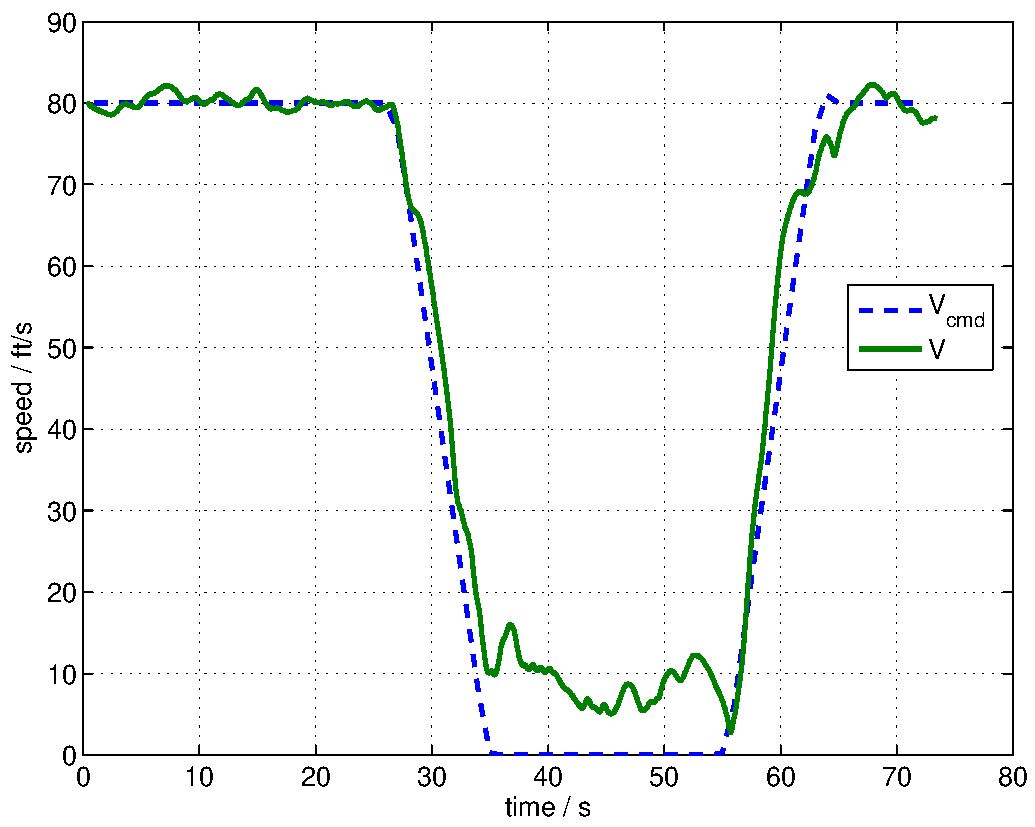
\includegraphics[height=\myfigheight]{edgeTransitionSpeed}
  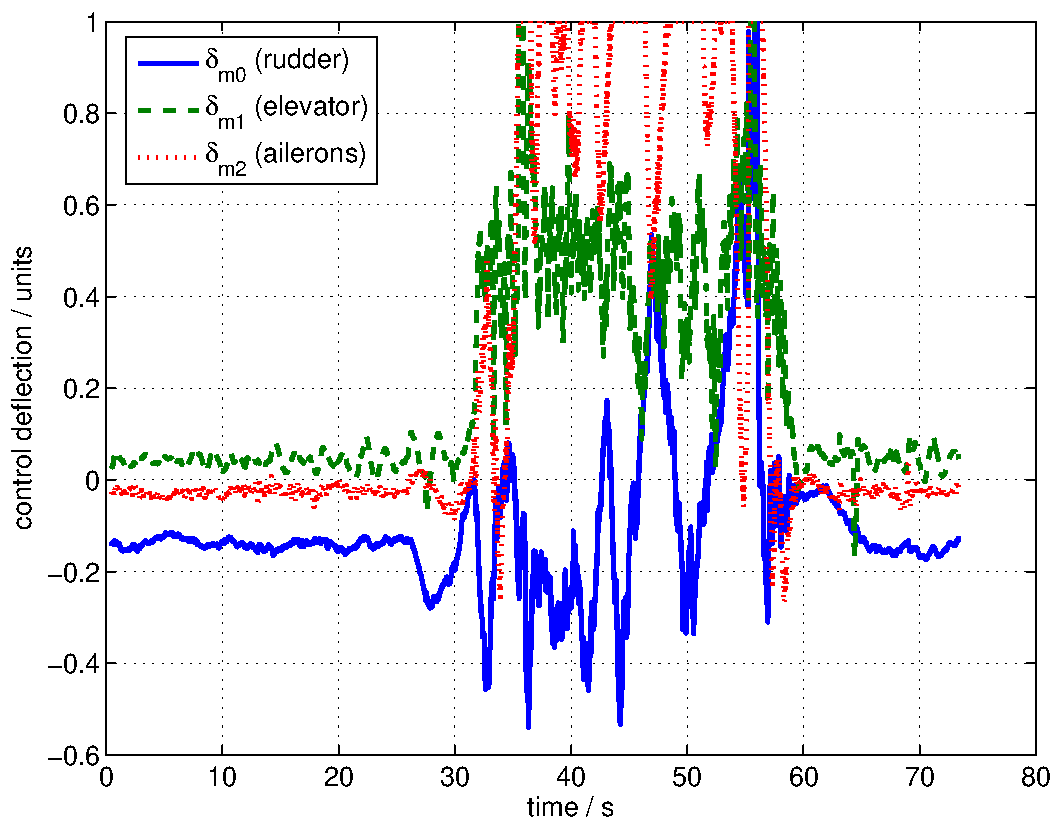
\includegraphics[height=\myfigheight]{edgeTransitionMomentControls}
  \caption{GTEdge speed profile and control deflections during transitions between hover and forward flight}
  \label{f:gtedgeSpeedMomentControls}
  \end{center}
\end{figure}

The following figures illustrate the response of the aircraft during
transitions between hover and forward flight.
\fig{f:gtedgeSpeedMomentControls} shows the vehicle in forward
flight at $80 ft/s$ performing a circular orbit. At $t = 26s$ a
transition to hover is initiated by supplying external trajectory
commands that lower the vehicle's speed. Transition is completed at
$t = 35 s$ with a low residual speed of approximately $5 ft/s$. At
$t = 55 s$ a transition back to forward flight at $80 ft/s$ is
initiated and completed at $t = 65 s$. During hover, $t\in[35,55]$,
the control deflections are seen to be significantly higher due to
the lower effectiveness at lower speeds. The ailerons are saturated
for significant intervals in a particular direction in order to
counteract engine torque.


\fig{f:gtedgePitchThrottle} illustrates the (helicopter) pitch angle
during transitions as well as the throttle control deflections. In
forward flight, the pitch angle is approximately $-75 deg$ and
varies in hover due to reduced control effectiveness and the
presence of a steady wind. Additionally, \fig{f:gtedgeTrajectory}
shows the position trajectory during transitions whereas
\fig{f:gtedgeDuringTransition} is a snapshot of the aircraft during
the maneuver.

\begin{figure}
  \begin{center}
  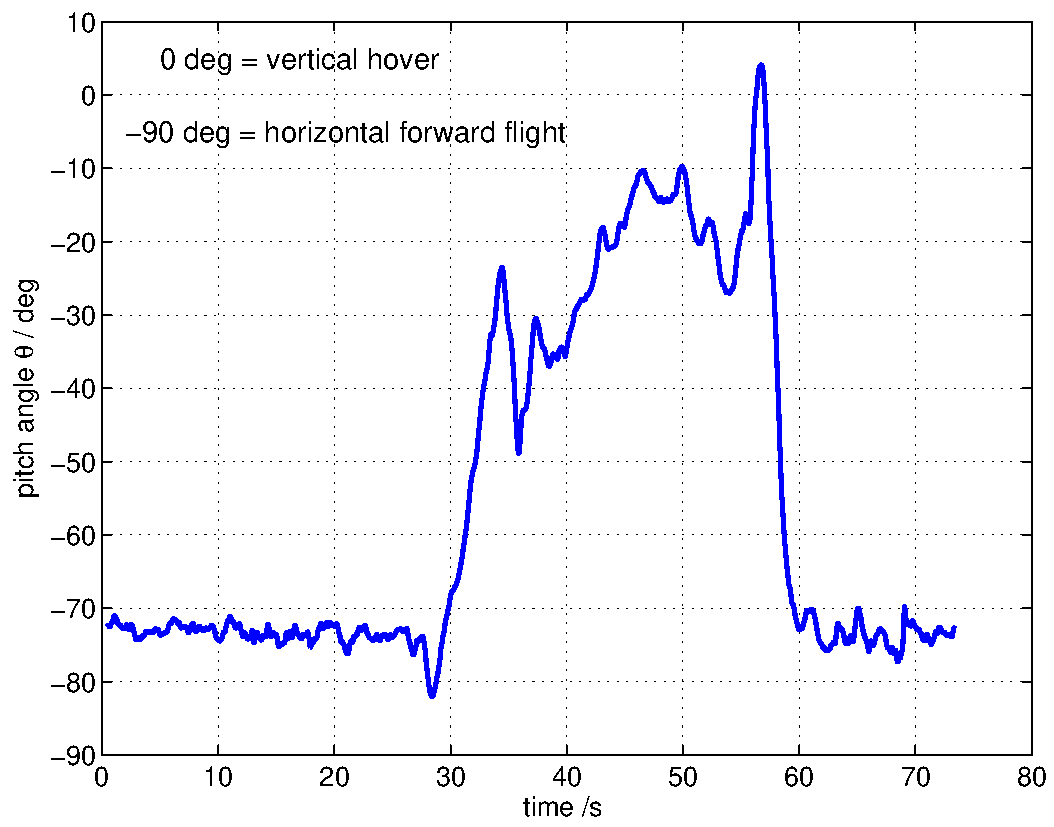
\includegraphics[height=\myfigheight]{edgeTransitionPitchAngle}
  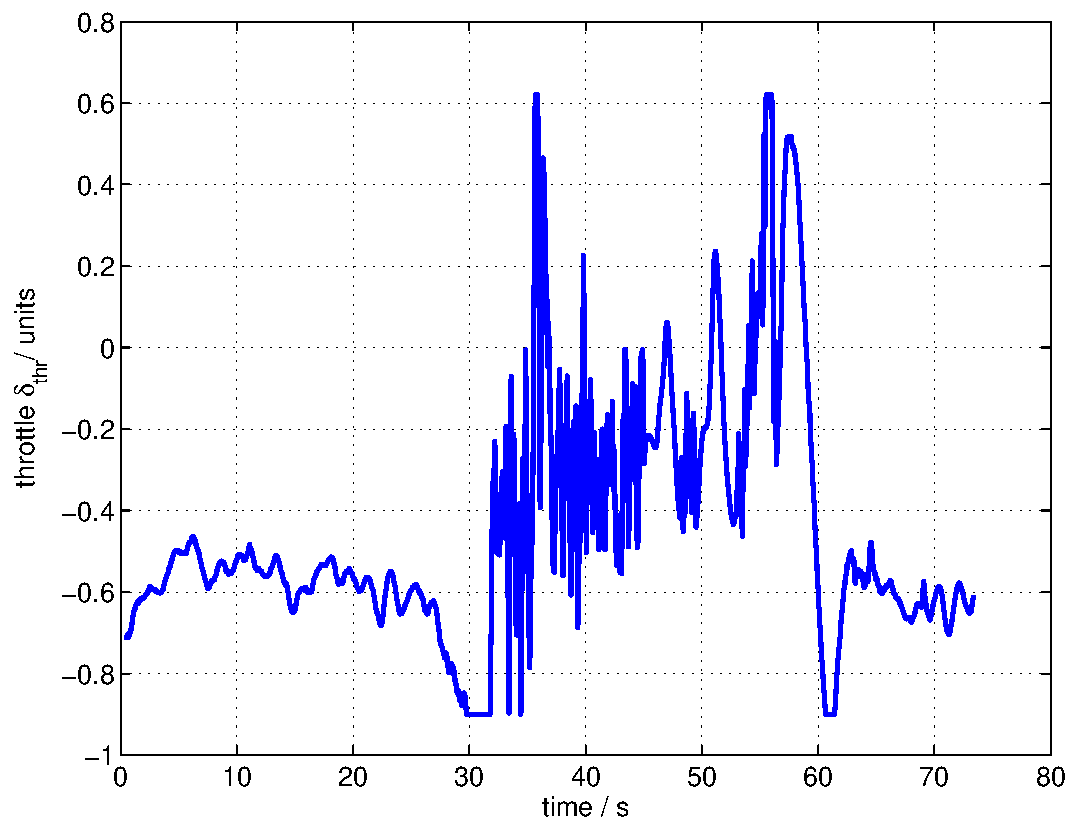
\includegraphics[height=\myfigheight]{edgeTransitionThrottle}
  \caption{GTEdge pitch angle, throttle profile during transitions between hover and forward flight}
  \label{f:gtedgePitchThrottle}
  \end{center}
\end{figure}

\begin{figure}
  \begin{center}
  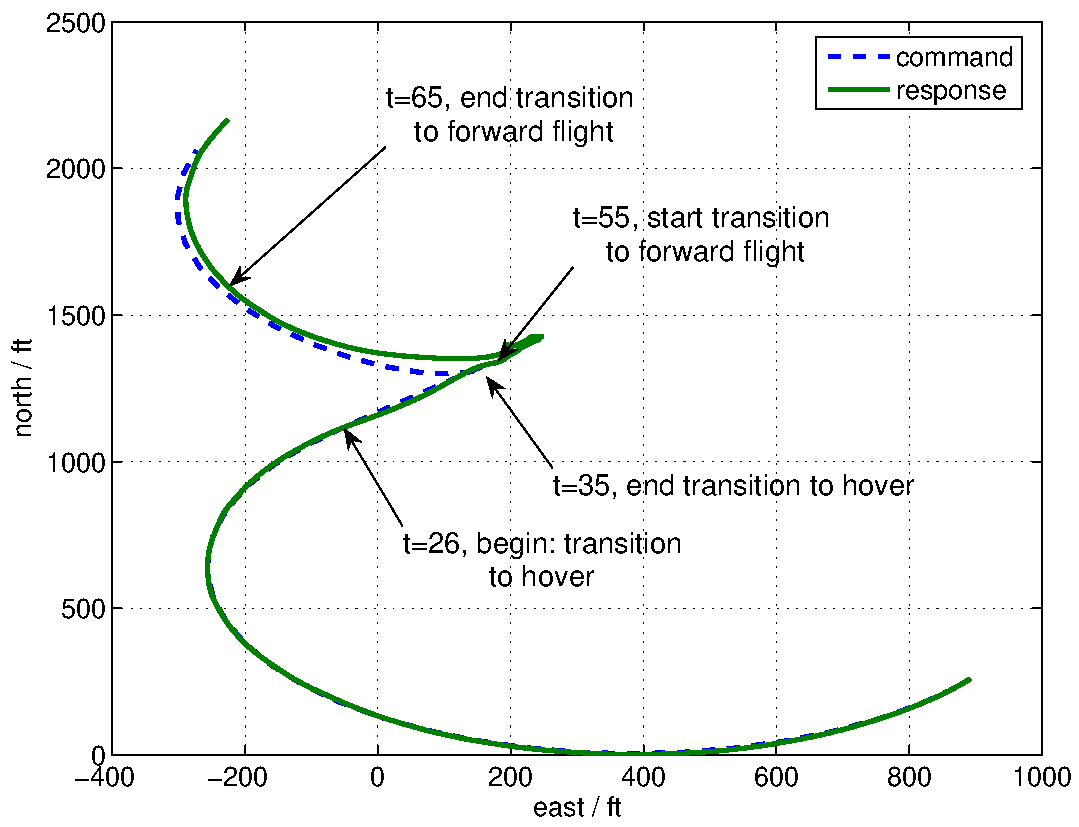
\includegraphics[height=\myfigheight]{edgeTransitionNorthEastPlanView}
  \caption{GTEdge trajectory during transitions}
  \label{f:gtedgeTrajectory}
  \end{center}
\end{figure}

\begin{figure}
  \begin{center}
  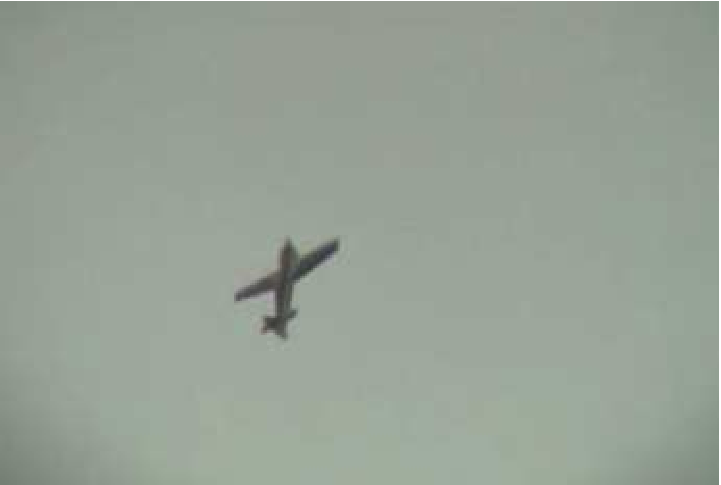
\includegraphics[height=\myfigheight]{edgeDuringTransition}
  \caption{GTEdge during a transition}
  \label{f:gtedgeDuringTransition}
  \end{center}
\end{figure}

\todo{Shorten the subsection titles and perhaps  make subusb section into a subsection}
\subsection{Implementation of Concurrent Learning Adaptive Controller on a VTOL UAV}\label{s:conc_flight_test}
\todo[inline,color=green]{Some of this section is redundant, we should refer back to previous descriptions of the experimental setup, or simply not mention it because it will just flow}
\todo[inline]{A little smoothing will fix disconnect}
Flight-test results of the concurrent learning adaptive law described in Section \ref{s:conc} are presented in this section. The test vehicle is the GTMax rotorcraft UAV. The modification to the adaptive controller described in Section \ref{s:controller} include the concurrent learning adaptive law of Equations \ref{eq:bg_learninglaw} for a nonlinearly parameterized SHL NN. Data points were selected online based on Equation \ref{eq:points_criterion} and were stored in a history stack limited to carrying $20$ points. Once the history stack was full,  a new data point was added by replacing the oldest data point. A fixed point smoother was used to estimate $\dot x_j$ for a recorded data point using both forward and a backward Kalman filter \cite{Chowdhary:JGCD:10,Gelb:74bk}. Typically this induced a selectable time-delay introduced by the time required for the smoother to converge, however, this does not affect the instantaneous tracking error.

\subsubsection{Repeated Forward Step Maneuvers}
\label{sec:bg_steps}
The repeated forward step maneuvers are chosen in order to create a relatively simple situation in which the controller performance can be compared over several similar maneunvers. By using concurrent learning NN improved performance is expected through repeated maneuvers and a faster convergence of weights. Figure \ref{fig:steps_all_states}  shows the body frame states from recorded flight data for a chain of forward step inputs. Figure \ref{fig:steps_errors_il_bg} and Figure \ref{fig:steps_errors_ol_bg} shows the evolution of inner and outer loop errors. These results assert the stability (in the ultimate boundedness sense) of the combined concurrent and online learning approach.

Figure \ref{fig:steps_W_bg} and Figure \ref{fig:steps_V_bg} show the evolution of NN $W$ and $V$ weights as the rotorcraft performs repeated step maneuvers and the NN is trained using the concurrent learning method of Theorem \ref{th:bg_bounded}. The NN $V$ weights (\ref{fig:steps_V_bg}) appear to go to constant values when concurrent learning adaptation is used, this can be contrasted with Figure \ref{fig:steps_V_o} which shows the $V$ weight adaptation for a similar maneuver without concurrent learning. NN $W$ weights for both cases remain bounded, however it is seen that with concurrent learning adaptation the NN $W$ weights seem to separate, this indicates alleviation of the rank-1 condition experienced by the baseline adaptive law relying only on instantaneous data \cite{Chowdhary:JGCD:10}. The flight test results indicate a noticeable improvement in the error profile. In Figure \ref{fig:steps_all_states} it is seen that the UAV tends not to have a smaller component of body lateral velocity ($v$) through each successive step. This is also seen in Figure \ref{fig:steps_errors_ol_bg}  where it is noted that the error in $v$ (body $y$ axis velocity) reduces through successive steps.  These effects in combination indicate that the combined online and concurrent learning system is able to improve performance over the baseline controller through repeated maneuvers, indicating long term learning.  These results are of particular interest, since the maneuvers performed were conservative, and the baseline adaptive MRAC controller had already been extensively tuned.



\begin{figure}[H]
\centering
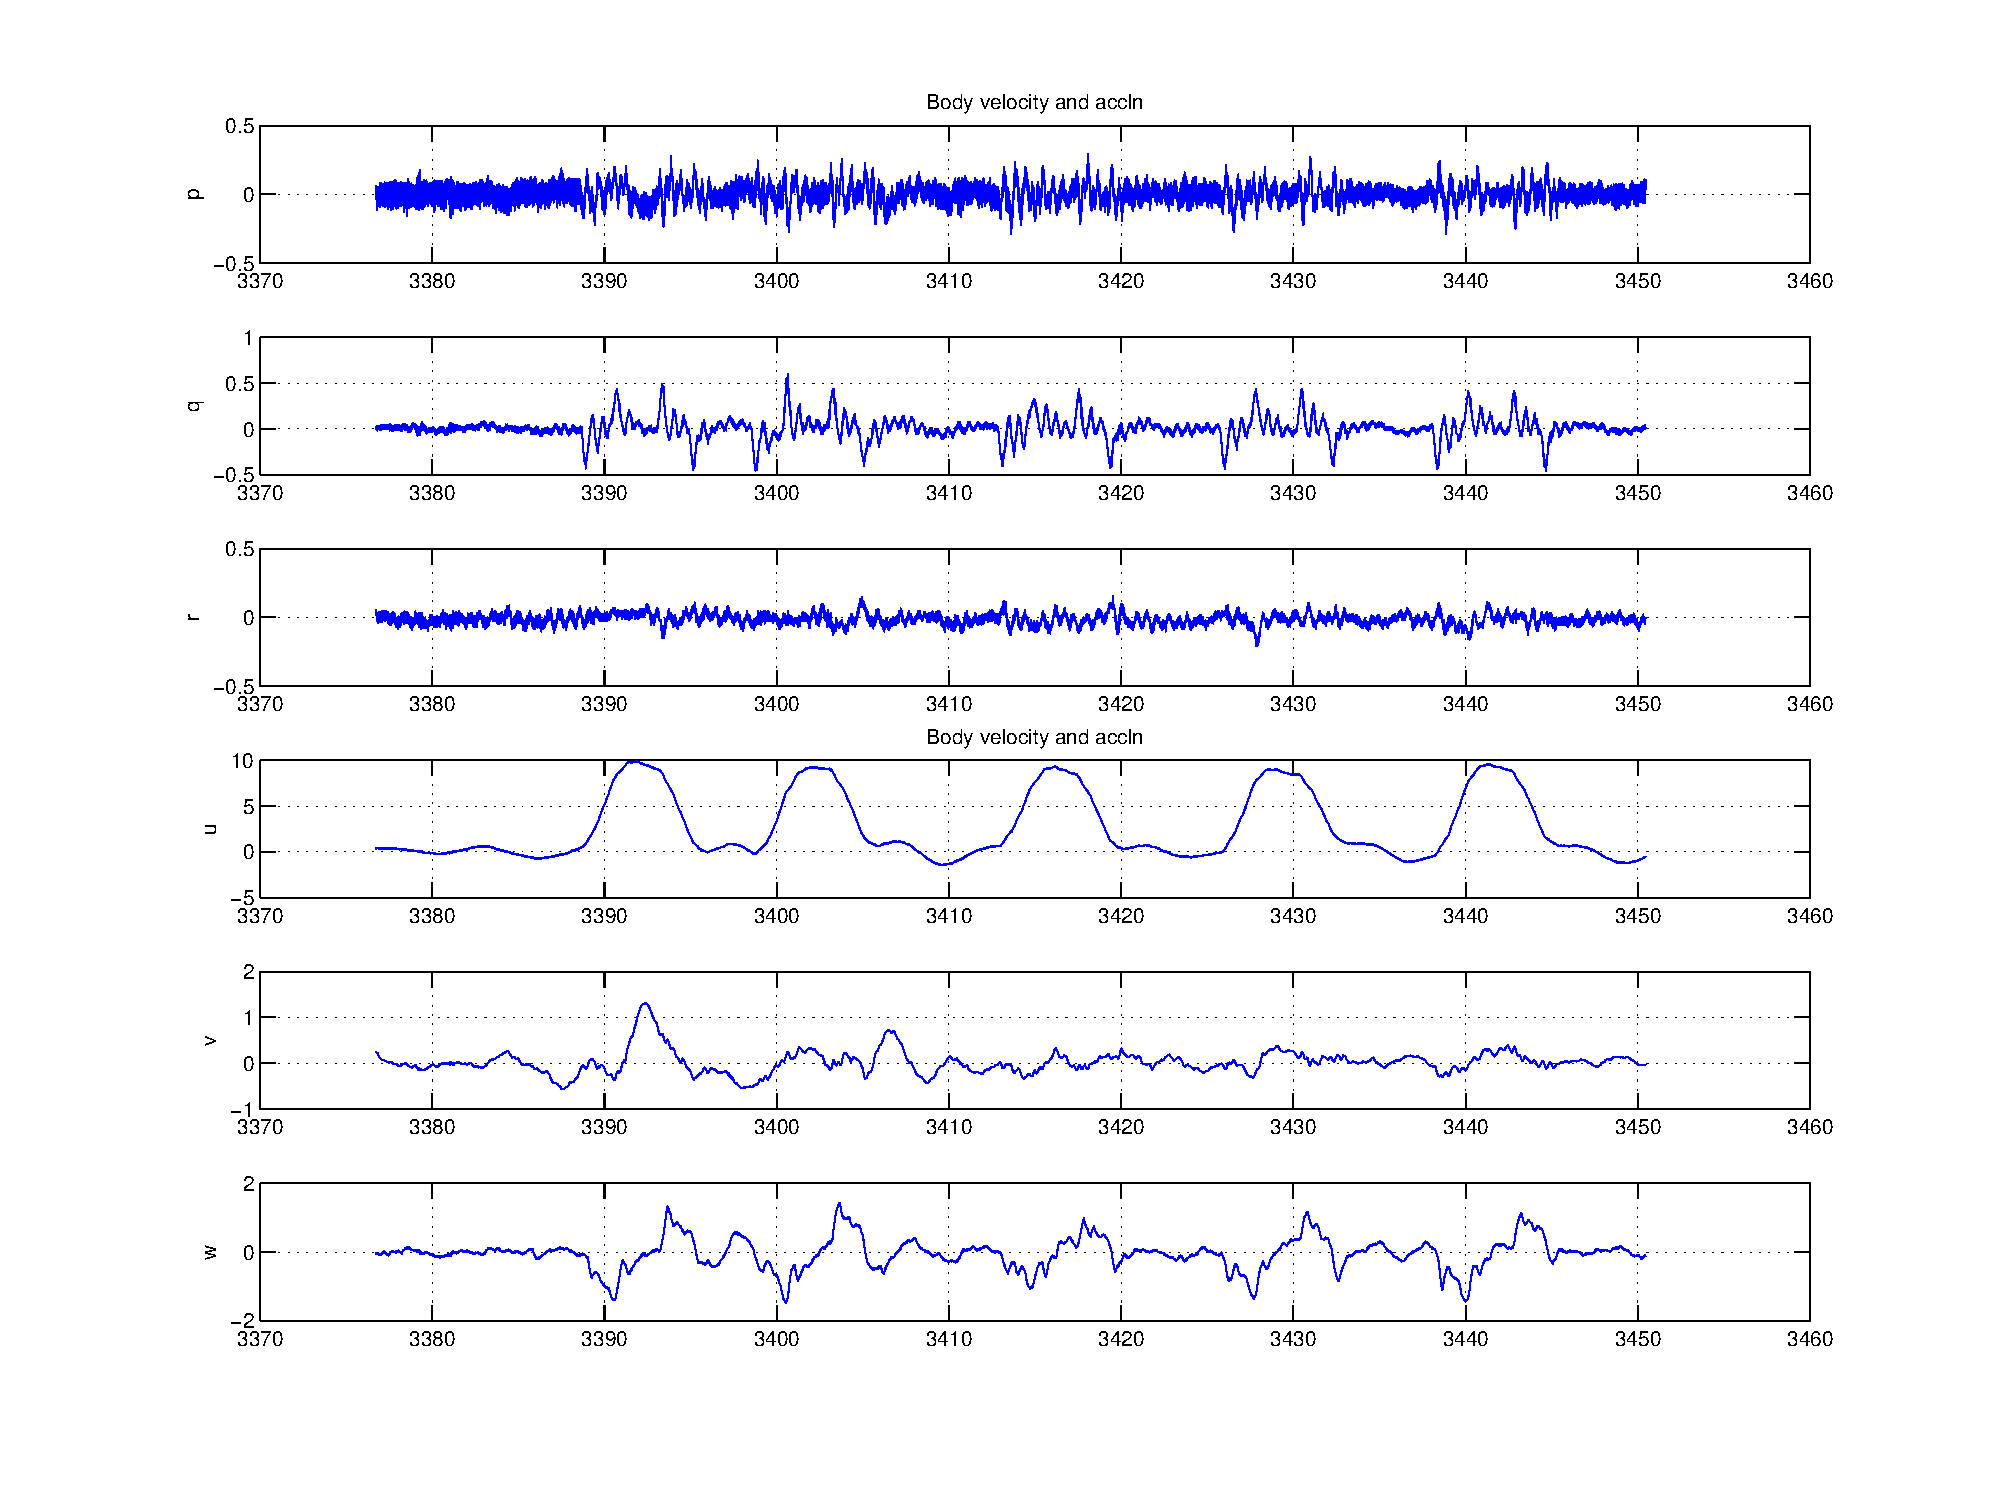
\includegraphics[scale=0.5]{steps_all_states}
\caption{Recorded Body Frame States for Repeated Forward Steps}
\label{fig:steps_all_states}
\end{figure}

\begin{figure}[H]
\centering
\subfigure[Evolution of inner loop errors with concurrent Adaptation]{\label{fig:steps_errors_il_bg}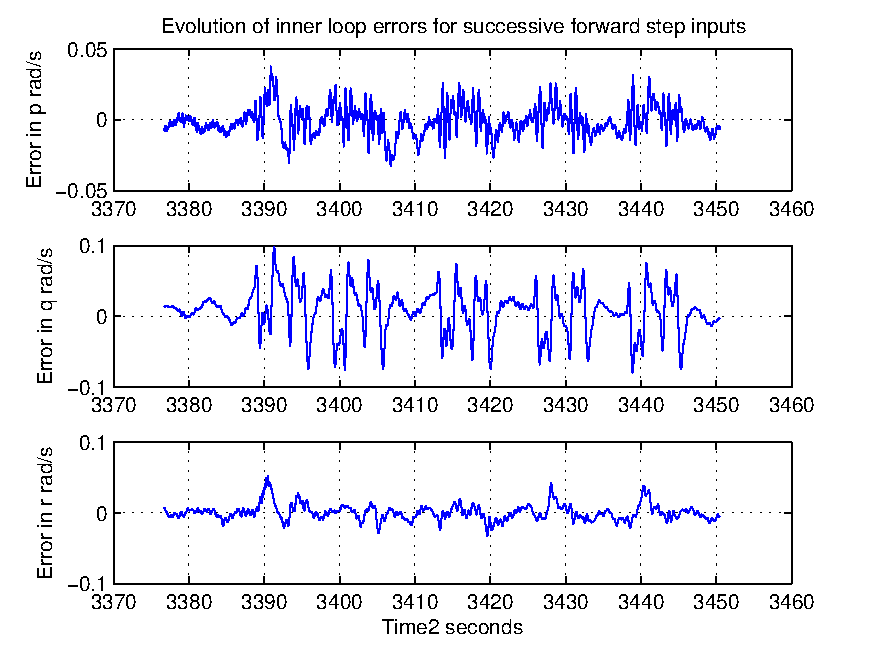
\includegraphics[scale=0.5]{steps_bg_il_errors}}
\subfigure[Evolution of outer loop errors with concurrent Adaptation]{\label{fig:steps_errors_ol_bg}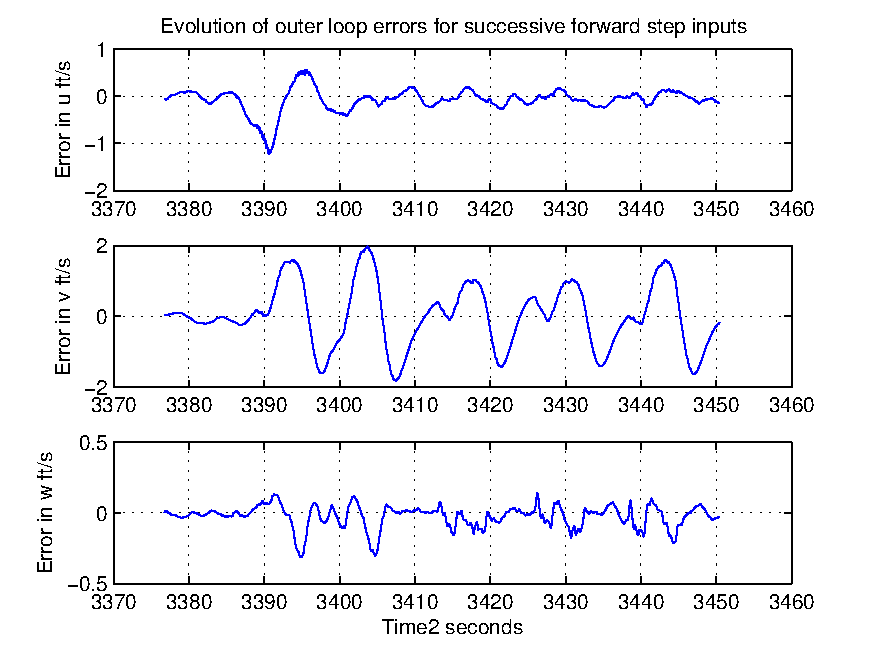
\includegraphics[scale=0.5]{steps_bg_ol_errors}}
\caption{GTMax Recorded Tracking Errors for Successive Forward Step Inputs with concurrent Learning}
\label{fig:steps_errors}
\end{figure}


\begin{figure}[H]
\centering
\subfigure[Evolution of $V$ matrix weights with Only Online Adaptation]{\label{fig:steps_V_o}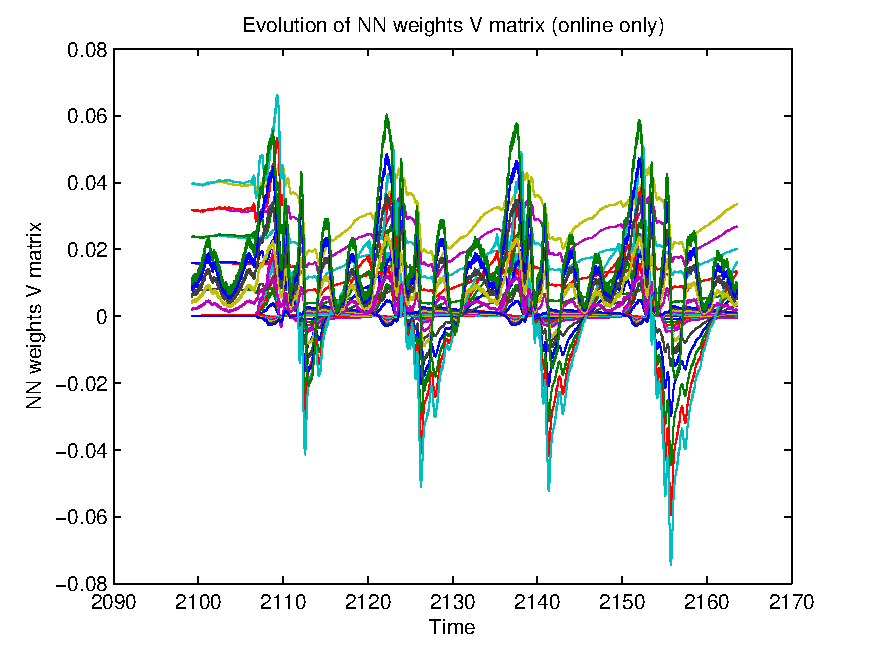
\includegraphics[scale=0.5]{sim_online_v}}
\subfigure[Evolution of $V$ matrix weights with concurrent Adaptation]{\label{fig:steps_V_bg}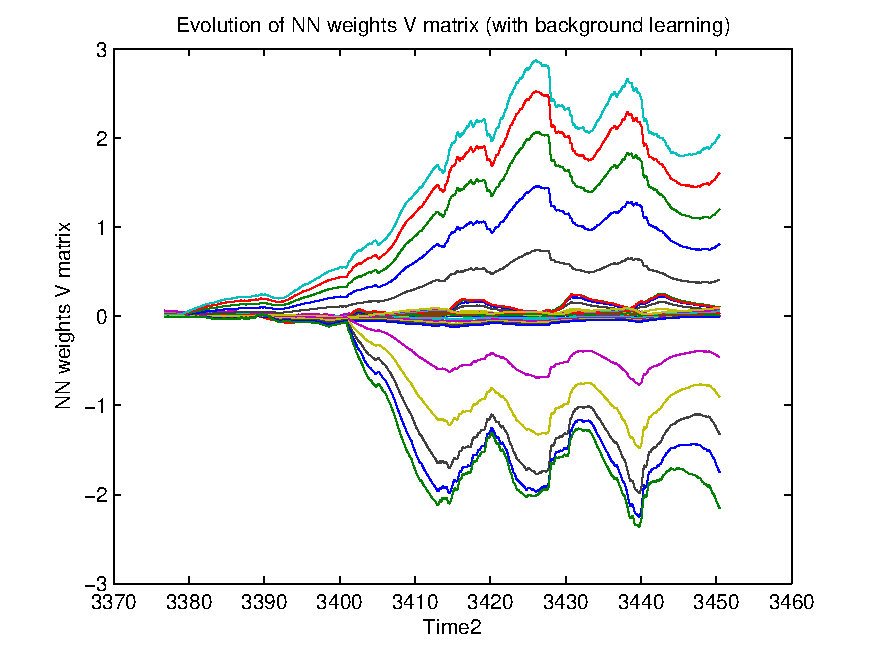
\includegraphics[scale=0.5]{steps_bg_V}}
\subfigure[Evolution of $W$ matrix weights with Only Online Adaptation]{\label{fig:steps_W_o}\includegraphics[scale=0.5]{sim_online_w}}
\subfigure[Evolution of $W$ matrix weights with concurrent Adaptation]{\label{fig:steps_W_bg}\includegraphics[scale=0.5]{steps_bg_W}}
\caption{Comparison of Weight Convergence on GTMax with and without concurrent Learning}
\label{fig:steps_weights}
\end{figure}
%%
\subsubsection{Aggressive Trajectory Tracking Maneuvers}
Flight-test results are presented for concurrent learning adaptive controllers while tracking repeatedly an elliptical trajectory with aggressive velocity ($50 ft/s$) and acceleration ($~20 ft/s^2$) profile. Since these maneuvers involve state commands in more than one system state it is harder to visually inspect the data and see whether an improvement in performance is seen, therefore the Euclidian norm of the error signal at each time step is used as a rudimentary metric. Figure \ref{fig:all_states_agg_ovals} shows the recorded inner and outer loop states as the rotorcraft repeatedly tracks an oval trajectory pattern. In this flight, the first two ovals (until t = 5415 s) are tracked with a commanded acceleration of $30ft/sec^2$, while the rest of the ovals are tracked at $20ft/sec^2$. In the following both these parts of the flight test are discussed separately.

\subsubsection{Aggressive Trajectory Tracking with Saturation in the Collective Channel}
\label{sec:bg_oval}
Due to the aggressive acceleration profile of $30ft/s^2$ the rotorcraft collective channels were observed to saturate while performing high velocity turns. This leads to an interesting challenge for the adaptive controller equipped with pseudo-control hedging. Figure \ref{fig:oval_sat_errors} shows the evolution of the innerloop and outerloop tracking error. It can be clearly seen that the tracking error in the $u$ (body x axis velocity) channel reduces in the second pass through the ellipse indicating long term learning by the combined online and concurrent learning adaptive control system. This result is further characterized by the noticeable reduction in the norm of the tracking error at every time step as shown in Figure \ref{fig:bg_agg_Sat_error_norm} \todo{this should reference something 24 is hardcoded}.



\begin{figure}[H]
\centering
\includegraphics[scale=0.6]{all_states_agg_oval}
\caption{Recorded Body Frame States for Repeated Oval Maneuvers}
\label{fig:all_states_agg_ovals}
\end{figure}

\begin{figure}[H]
\centering
\subfigure[Evolution of inner loop errors with concurrent Adaptation]{\label{fig:bg_agg_sat_il_e}\includegraphics[scale=0.5]{bg_agg_sat_il_e}}
\subfigure[Evolution of outer loop errors with concurrent Adaptation]{\label{fig:bg_agg_sat_ol_e}\includegraphics[scale=0.5]{bg_agg_sat_ol_e}}
\caption{GTMax Recorded Tracking Errors for Aggressive Maneuvers with Saturation in Collective Channels with concurrent Learning}
\label{fig:oval_sat_errors}
\end{figure}

\begin{figure}[H]
\centering
\includegraphics[scale=0.7]{bg_agg_sat_error_norm}
\caption{Plot of the norm of the error at each time step for aggressive trajectory tracking with collective saturation}
\label{fig:bg_agg_Sat_error_norm}
\end{figure}

\subsubsection{Aggressive Trajectory Tracking Maneuver}
For the results presented in this section, the acceleration profile was reduced to $20ft/sec^2$. At this acceleration profile, no saturation in the collective input was noted. Figure \ref{fig:oval_nosat_errors} shows the evolution of tracking error, and Figure \ref{fig:bg_agg_nosat_error_norm} shows the plot of the norm of the tracking error at each time step.
\begin{figure}[H]
\centering
\subfigure[Evolution of inner loop errors with concurrent Adaptation]{\label{fig:bg_agg_nosat_il_e}\includegraphics[scale=0.5]{bg_agg_nosat_il_e}}
\subfigure[Evolution of outer loop errors with concurrent Adaptation]{\label{fig:bg_agg_nosat_ol_e}\includegraphics[scale=0.5]{bg_agg_nosat_ol_e}}
\caption{GTMax Recorded Tracking Errors for Aggressive Maneuvers with concurrent Learning}
\label{fig:oval_nosat_errors}
\end{figure}

\begin{figure}[H]
\centering
\subfigure[Evolution of the norm of the tracking error with concurrent Adaptation]{\label{fig:bg_agg_nosat_error_norm}\includegraphics[scale=0.42]{bg_agg_nosat_error_norm}}
\subfigure[Evolution of the norm of the tracking error with only online Adaptation]{\label{fig:o_agg_nosat_error_norm}\includegraphics[scale=0.5]{online_agg_nosat_error_norm}}
\caption{Comparison of norm of GTMax Recorded Tracking Errors for Aggressive Maneuvers}
\label{fig:oval_comparision_error_norm}
\end{figure}

\subsubsection{Aggressive Trajectory Tracking Maneuvers with Only Online Learning NN}
The performance of the concurrent learning adaptive controller is compared with the traditional instantaneous update based adaptive controllers for the maneuvers described in Section \ref{sec:bg_oval}.

It is instructive to compare Figure \ref{fig:oval_V_bg}, and Figure \ref{fig:oval_W_bg} which show the evolution of the NN weights with only instantaneous learning with Figure \ref{fig:oval_V_o}, and Figure \ref{fig:oval_W_o} which show evolution of the NN weights with concurrent learning. Although absolute convergence of weights is not seen, as expected due to Theorem \ref{th:bg_bounded} it is interesting to see that when concurrent learning is on, the weights tend to be less oscillatory than when only instantaneous learning is used. Also, with combined online and concurrent learning, the weights do not tend to go to zero as the rotorcraft hovers between two successive tracking maneuver. Figure \ref{fig:o_agg_nosat_error_norm} shows the plot of the tracking error norm as a function of time without concurrent learning. Comparing this figure with Figure \ref{fig:bg_agg_nosat_error_norm} it can be clearly seen that the norm of the error vector is much higher when only online learning is used. This indicates that the combined online and concurrent learning adaptive controller has improved trajectory tracking performance.
\begin{figure}[H]
\centering
\subfigure[Evolution of $V$ matrix weights with Only Online Adaptation]{\label{fig:oval_V_o}\includegraphics[scale=0.5]{online_agg_nosat_V}}
\subfigure[Evolution of $V$ matrix weights with concurrent Adaptation]{\label{fig:oval_V_bg}\includegraphics[scale=0.5]{bg_agg_nosat_V}}
\subfigure[Evolution of $W$ matrix weights with Only Online Adaptation]{\label{fig:oval_W_o}\includegraphics[scale=0.5]{online_agg_nosat_W}}
\subfigure[Evolution of $W$ matrix weights with concurrent Adaptation]{\label{fig:oval_W_bg}\includegraphics[scale=0.5]{bg_agg_nosat_W}}
\caption{Comparison of Weight Convergence as GTMax tracks aggressive trajectory with and without concurrent Learning }
\label{fig:oval_weights}
\end{figure}
In summary, the flight test results ascertain an expected improvement in tracking performance.  Furthermore, the evolution of the neural network W and V matrix weights were observed to have different characteristics when concurrent learning was employed, including, weight separation, a tendency towards weight convergence in some cases, and different numerical values of the adaptive weights. This difference in neural network weight behavior demonstrates the effect of overcoming the rank-1 condition.

